\section{Mục tiêu xây dựng các mô hình}

Sau quá trình phân tích khám phá dữ liệu và trực quan hóa, em tiếp tục xây dựng các mô hình phân tích dữ liệu nhằm khai thác sâu hơn mối quan hệ giữa các biến trong bộ dữ liệu Superstore Sales, hướng đến việc xây dựng các mô hình thực nghiệm nhằm dự báo lợi nhuận và phân tích đặc điểm tiêu dùng của khách hàng.

Lợi nhuận là chỉ tiêu phản ánh trực tiếp hiệu quả kinh doanh, không chỉ thể hiện quy mô bán hàng mà còn cho biết mức độ sinh lời sau khi xét đến các yếu tố như chiết khấu, số lượng bán, nhóm sản phẩm và khu vực bán hàng. Do đó, việc dự báo lợi nhuận có ý nghĩa quan trọng trong việc hỗ trợ doanh nghiệp đánh giá hiệu quả hoạt động kinh doanh.

Mục tiêu chính của quá trình xây dựng mô hình gồm:
\begin{itemize}
    \item Dự báo lợi nhuận dựa trên các yếu tố đầu vào như số lượng bán, chiết khấu, phương thức giao hàng, khu vực, danh mục sản phẩm và phân khúc khách hàng.
    \item So sánh hiệu quả giữa các mô hình học máy khác nhau trên cùng bộ dữ liệu.
    \item Đánh giá ảnh hưởng của việc xử lý giá trị ngoại lai đến hiệu quả dự báo của từng mô hình.
    \item Nhận diện mô hình phù hợp hơn đối với bài toán dự báo lợi nhuận trong dữ liệu bán lẻ.
    \item Phân cụm khách hàng theo đặc điểm tiêu dùng nhằm hỗ trợ phân tích nhóm khách hàng.
\end{itemize}

Các mô hình được triển khai trong chương này gồm Hồi quy tuyến tính đa biến, Random Forest Regressor, Gradient Boosting Regressor, XGBoost Regressor và K-Means Clustering. Trong đó, bốn mô hình đầu tiên được sử dụng cho bài toán dự báo lợi nhuận, còn K-Means được sử dụng cho bài toán phân cụm khách hàng.

Quy trình xây dựng mô hình được thực hiện qua các bước chính: xác định mục tiêu phân tích, thu thập dữ liệu, làm sạch dữ liệu, xây dựng mô hình, thực hiện đánh giá mô hình, cải tiến mô hình, triển khai vào thực tế, theo dõi hiệu quả thực hiện.

\begin{figure}[H]
    \centering
    
\includegraphics[width=0.85\textwidth]{images/anh_chuong4/model_workflow.png}
    \caption{Quy trình xây dựng và đánh giá mô hình phân tích dữ liệu}
    \label{fig:model_workflow}
\end{figure}

\section{Lựa chọn các biến phân tích}

Trong bài toán dự báo, biến mục tiêu được lựa chọn là \textbf{Profit}. Đây là biến phản ánh lợi nhuận thu được từ từng giao dịch và là chỉ tiêu quan trọng để đánh giá hiệu quả kinh doanh. Việc lựa chọn Profit làm biến mục tiêu giúp mô hình tập trung vào bài toán sinh lời thay vì chỉ dự báo quy mô doanh thu.

Các biến đầu vào được lựa chọn dựa trên đặc điểm của bộ dữ liệu và mục tiêu nghiên cứu, bao gồm:
\begin{itemize}
    \item \textbf{Quantity}: số lượng sản phẩm được bán trong mỗi giao dịch.
    \item \textbf{Discount}: mức chiết khấu được áp dụng.
    \item \textbf{Shipping Days}: số ngày giao hàng, được tính từ thời điểm đặt hàng đến thời điểm giao hàng.
    \item \textbf{Sales}: doanh thu của từng giao dịch.
    \item \textbf{Ship Mode}: phương thức giao hàng.
    \item \textbf{Segment}: phân khúc khách hàng.
    \item \textbf{Region}: khu vực bán hàng.
    \item \textbf{Category}: danh mục sản phẩm.
    \item \textbf{Sub-Category}: tiểu danh mục sản phẩm.
    \item \textbf{Year, Month, Quarter}: các biến thời gian được trích xuất từ ngày đặt hàng.
\end{itemize}

Một số biến định danh như \textit{Order ID}, \textit{Customer ID}, \textit{Customer Name}, \textit{Product ID} và \textit{Product Name} được loại bỏ khỏi tập dữ liệu đầu vào. Các biến này chủ yếu dùng để nhận diện đơn hàng, khách hàng hoặc sản phẩm cụ thể, không phản ánh trực tiếp quy luật dự báo lợi nhuận.

Đối với các biến định tính, đề tài sử dụng phương pháp One-Hot Encoding để chuyển đổi sang dạng số. Đây là bước cần thiết vì các mô hình học máy yêu cầu dữ liệu đầu vào ở dạng số. Đối với các biến số, dữ liệu được kiểm tra và xử lý ngoại lai bằng phương pháp IQR Capping trong trường hợp cần so sánh trước và sau xử lý ngoại lai.

Dữ liệu được chia thành hai phần:
\begin{itemize}
    \item Tập huấn luyện chiếm 80\% dữ liệu.
    \item Tập kiểm tra chiếm 20\% dữ liệu.
\end{itemize}

Việc chia dữ liệu thành tập huấn luyện và tập kiểm tra giúp đánh giá khả năng tổng quát hóa của mô hình. Nếu mô hình chỉ cho kết quả tốt trên tập huấn luyện nhưng kém trên tập kiểm tra, điều đó cho thấy mô hình có thể đang bị quá khớp với dữ liệu huấn luyện.

\begin{table}[H]
\centering
\caption{Các nhóm biến sử dụng trong quá trình xây dựng mô hình}
\label{tab:model_variables}
\begin{tabular}{|p{4cm}|p{8cm}|}
\hline
\textbf{Nhóm biến} & \textbf{Biến sử dụng} \\ \hline
Biến mục tiêu & Profit \\ \hline
Biến định lượng & Quantity, Discount, Shipping Days, Sales, Year, Month, Quarter \\ \hline
Biến định tính & Ship Mode, Segment, Region, Category, Sub-Category \\ \hline
Biến loại bỏ & Order ID, Customer ID, Customer Name, Product ID, Product Name \\ \hline
\end{tabular}
\end{table}

\section{Mô hình hồi quy tuyến tính đa biến}


\refstepcounter{subsection}
\subsection*{\thesubsection\quad Giới thiệu mô hình}


Hồi quy tuyến tính đa biến là mô hình cơ bản được sử dụng để mô tả mối quan hệ tuyến tính giữa nhiều biến độc lập và một biến phụ thuộc. Mô hình được sử dụng để dự báo lợi nhuận dựa trên các yếu tố như số lượng bán, chiết khấu, khu vực, phân khúc khách hàng, danh mục sản phẩm và thời gian giao hàng.

Mô hình hồi quy tuyến tính đa biến được lựa chọn làm mô hình cơ sở. Vai trò của mô hình này không chỉ là dự báo lợi nhuận mà còn giúp tạo ra một mốc so sánh ban đầu để đánh giá hiệu quả của các mô hình phức tạp hơn như Random Forest, Gradient Boosting và XGBoost.

Ưu điểm của mô hình hồi quy tuyến tính là dễ xây dựng, dễ diễn giải và phù hợp khi mối quan hệ giữa biến đầu vào và biến mục tiêu có xu hướng tuyến tính. Tuy nhiên, trong dữ liệu kinh doanh bán lẻ, mối quan hệ giữa các biến thường phức tạp hơn. Ví dụ, chiết khấu có thể giúp tăng doanh thu nhưng đồng thời làm giảm lợi nhuận. Vì vậy, mô hình hồi quy tuyến tính có thể gặp hạn chế khi áp dụng vào bài toán này.

\refstepcounter{subsection}
\subsection*{\thesubsection\quad Kết quả trước xử lý ngoại lai}

Trước khi xử lý giá trị ngoại lai, mô hình hồi quy tuyến tính đa biến cho kết quả thấp trên cả tập huấn luyện và tập kiểm tra. 

Cụ thể:
\begin{itemize}
	\item Tập huấn luyện đạt \(MAE = 74.2328\), \(RMSE = 223.1231\) và \(R^2 = 0.199\).
	\item Tập kiểm tra đạt \(MAE = 73.6679\), \(RMSE = 144.649\) và \(R^2 = 0.0305\).
\end{itemize}

Giá trị \(R^2\) trên tập kiểm tra rất thấp cho thấy mô hình gần như chưa giải thích được sự biến động của lợi nhuận trong dữ liệu kiểm tra. Điều này phản ánh khả năng dự báo của mô hình còn hạn chế khi dữ liệu vẫn tồn tại nhiều điểm ngoại lai.

\begin{figure}[H]
	\centering
	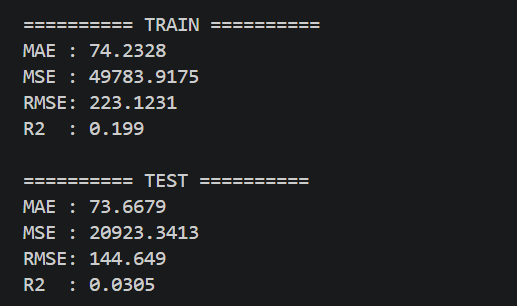
\includegraphics[width=0.6\textwidth]{images/anh_chuong4/linear_before_metrics.png}
	\caption{Kết quả mô hình hồi quy tuyến tính trước xử lý ngoại lai}
	\label{fig:linear_before_metrics}
\end{figure}

Nguyên nhân chủ yếu đến từ đặc điểm của dữ liệu bán lẻ. Bộ dữ liệu Superstore Sales có sự chênh lệch lớn giữa các giao dịch. Phần lớn các giao dịch có doanh thu và lợi nhuận ở mức trung bình hoặc thấp, trong khi một số giao dịch có lợi nhuận âm rất lớn hoặc lợi nhuận dương bất thường.


\begin{figure}[H]
	\centering
	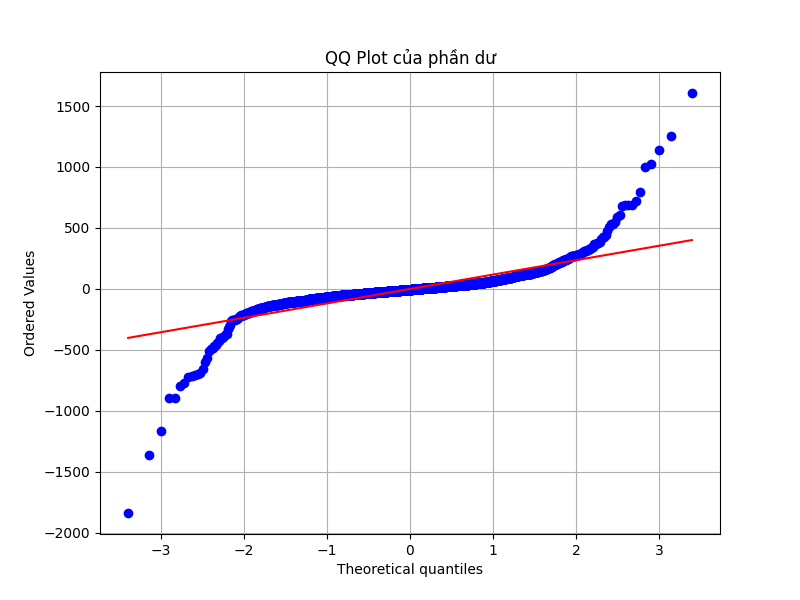
\includegraphics[width=0.75\textwidth]{images/anh_chuong4/linear_before_qqplot.png}
	\caption{QQ Plot phần dư trước xử lý ngoại lai}
	\label{fig:linear_before_qqplot}
\end{figure}

Quan sát QQ Plot trong Hình \ref{fig:linear_before_qqplot} cho thấy các điểm dữ liệu lệch khá xa khỏi đường thẳng chuẩn ở hai đầu phân phối. Điều này chứng tỏ phần dư của mô hình chưa tuân theo phân phối chuẩn và vẫn chịu ảnh hưởng mạnh của các giá trị ngoại lai.


\refstepcounter{subsection}
\subsection*{\thesubsection\quad Kết quả sau khi xử lý ngoại lai}

Sau khi áp dụng phương pháp IQR Capping để xử lý giá trị ngoại lai, hiệu quả của mô hình hồi quy tuyến tính đa biến được cải thiện rõ rệt trên cả tập huấn luyện và tập kiểm tra.

Cụ thể:
\begin{itemize}
	\item Tập huấn luyện đạt \(MAE = 16.8002\), \(RMSE = 21.3793\) và \(R^2 = 0.4707\).
	\item Tập kiểm tra đạt \(MAE = 18.4952\), \(RMSE = 23.4194\) và \(R^2 = 0.3617\).
\end{itemize}

So với trước khi xử lý ngoại lai, giá trị \(R^2\) trên tập kiểm tra đã tăng mạnh từ 0.0305 lên 0.3617. Đồng thời, các chỉ số MAE và RMSE giảm đáng kể. Điều này cho thấy việc xử lý ngoại lai giúp mô hình học tốt hơn xu hướng chung của dữ liệu và cải thiện đáng kể khả năng dự báo lợi nhuận.

\begin{figure}[H]
	\centering
	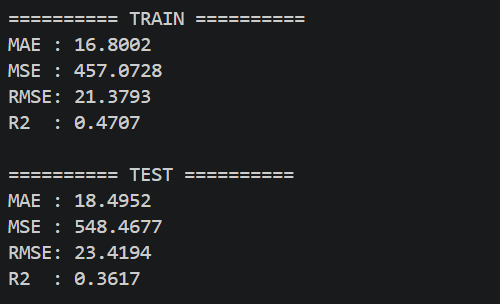
\includegraphics[width=0.6\textwidth]{images/anh_chuong4/linear_after_metrics.png}
	\caption{Kết quả mô hình hồi quy tuyến tính sau xử lý ngoại lai}
	\label{fig:linear_after_metrics}
\end{figure}

Nguyên nhân của sự cải thiện này là do các giá trị lợi nhuận quá lớn hoặc quá nhỏ đã được giới hạn trong khoảng hợp lý hơn. Việc giảm ảnh hưởng của các giao dịch bất thường giúp dữ liệu ổn định hơn và làm cho đường hồi quy phản ánh chính xác hơn xu hướng của phần lớn dữ liệu.



\begin{figure}[H]
	\centering
	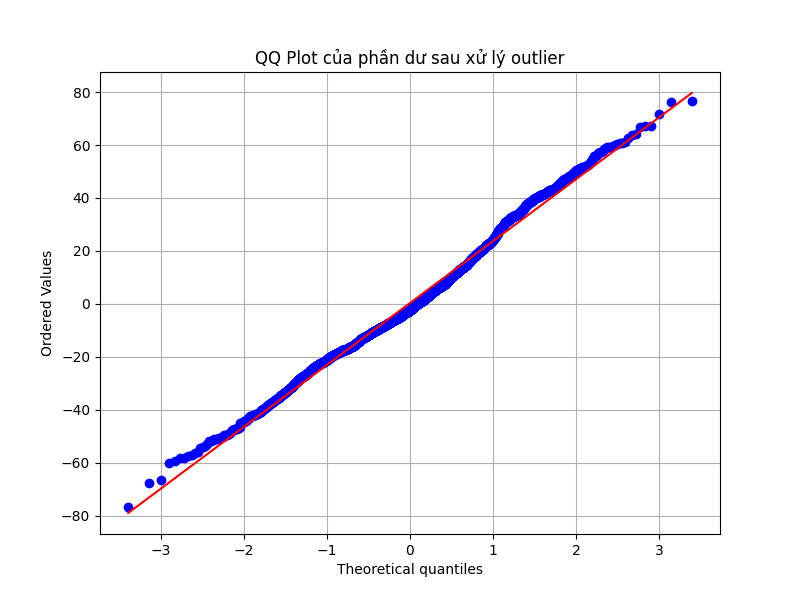
\includegraphics[width=0.75\textwidth]{images/anh_chuong4/linear_after_qqplot.png}
	\caption{QQ Plot phần dư sau xử lý ngoại lai}
	\label{fig:linear_after_qqplot}
\end{figure}

Quan sát QQ Plot trong Hình \ref{fig:linear_after_qqplot} cho thấy các điểm dữ liệu bám sát đường chuẩn hơn đáng kể so với trước khi xử lý ngoại lai. Điều này chứng tỏ phần dư của mô hình đã gần với phân phối chuẩn hơn.

Mặc dù ở hai đầu phân phối vẫn còn một số điểm lệch khỏi đường chuẩn, tuy nhiên mức độ lệch đã giảm rõ rệt. Điều này cho thấy việc xử lý ngoại lai đã giúp mô hình hồi quy tuyến tính hoạt động ổn định hơn và nâng cao khả năng dự báo trên bộ dữ liệu bán lẻ.

\refstepcounter{subsection}
\subsection*{\thesubsection\quad So sánh trước và sau xử lý ngoại lai}

Kết quả thực nghiệm cho thấy việc xử lý ngoại lai giúp cải thiện đáng kể hiệu quả của mô hình hồi quy tuyến tính đa biến. Sau khi áp dụng phương pháp IQR Capping, giá trị \(R^2\) trên tập kiểm tra tăng từ 0.0305 lên 0.3617, đồng thời các chỉ số MAE và RMSE giảm rõ rệt.

Điều này cho thấy các giá trị ngoại lai đã ảnh hưởng mạnh đến đường hồi quy và làm giảm khả năng dự báo của mô hình. Sau khi xử lý ngoại lai, dữ liệu trở nên ổn định hơn, giúp mô hình học tốt hơn xu hướng chung của dữ liệu.

\refstepcounter{subsection}
\subsection*{\thesubsection\quad Nhận xét mô hình}

Sau khi xử lý ngoại lai, hiệu quả mô hình được cải thiện rõ rệt, cho thấy hồi quy tuyến tính khá nhạy cảm với các giá trị bất thường trong dữ liệu.

Tuy nhiên, kết quả dự báo vẫn thấp hơn các mô hình học máy phi tuyến do dữ liệu bán lẻ tồn tại nhiều quan hệ và tương tác phức tạp giữa các biến. Vì vậy, mô hình hồi quy tuyến tính chưa phải lựa chọn tối ưu cho bài toán dự báo lợi nhuận, nhưng vẫn có ý nghĩa quan trọng trong việc làm cơ sở so sánh với các mô hình phức tạp, nâng cao hơn.

\section{Mô hình Random Forest}

\refstepcounter{subsection}
\subsection*{\thesubsection\quad Giới thiệu mô hình}

Random Forest Regressor là mô hình học máy thuộc nhóm ensemble learning. Mô hình hoạt động bằng cách xây dựng nhiều cây quyết định trên các mẫu dữ liệu khác nhau, sau đó lấy trung bình kết quả dự báo của các cây để đưa ra kết quả cuối cùng.

So với hồi quy tuyến tính, Random Forest có khả năng học các mối quan hệ phi tuyến tốt hơn. Mô hình không yêu cầu giả định rằng quan hệ giữa biến đầu vào và biến mục tiêu phải là tuyến tính. Đây là ưu điểm quan trọng khi áp dụng cho dữ liệu bán lẻ, nơi lợi nhuận có thể bị ảnh hưởng bởi nhiều yếu tố kết hợp với nhau.

\refstepcounter{subsection}
\subsection*{\thesubsection\quad Kết quả trước xử lý ngoại lai}

Trước khi xử lý giá trị ngoại lai, mô hình Random Forest cho kết quả tốt hơn mô hình hồi quy tuyến tính đa biến trên cả tập huấn luyện và tập kiểm tra.

Cụ thể:
\begin{itemize}
	\item Tập huấn luyện đạt \(MAE = 44.7721\), \(RMSE = 158.56\) và \(R^2 = 0.5955\).
	\item Tập kiểm tra đạt \(MAE = 56.1282\), \(RMSE = 138.8776\) và \(R^2 = 0.1063\).
\end{itemize}

Giá trị \(R^2\) trên tập kiểm tra cao hơn mô hình hồi quy tuyến tính, cho thấy Random Forest có khả năng học tốt hơn các quan hệ phi tuyến trong dữ liệu bán lẻ. Tuy nhiên, hiệu quả dự báo vẫn chưa cao do dữ liệu còn chứa nhiều giá trị ngoại lai.

\begin{figure}[H]
	\centering
	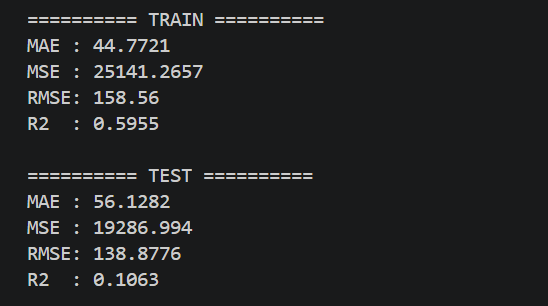
\includegraphics[width=0.6\textwidth]{images/anh_chuong4/random_forest_before_metrics.png}
	\caption{\centering Kết quả mô hình Random Forest trước xử lý ngoại lai}
	\label{fig:rf_before_metrics}
\end{figure}

Nguyên nhân chủ yếu đến từ đặc điểm của bộ dữ liệu Superstore Sales. Một số giao dịch có lợi nhuận quá lớn hoặc quá nhỏ làm tăng độ biến động của biến Profit và ảnh hưởng đến quá trình xây dựng cây quyết định.

Mặc dù Random Forest ít nhạy cảm với ngoại lai hơn hồi quy tuyến tính, mô hình vẫn có thể bị ảnh hưởng khi dữ liệu tồn tại nhiều giá trị cực đoan. Một số cây quyết định có xu hướng học quá chi tiết từ các giao dịch bất thường, làm giảm khả năng tổng quát hóa trên tập kiểm tra.

\begin{figure}[H]
	\centering
	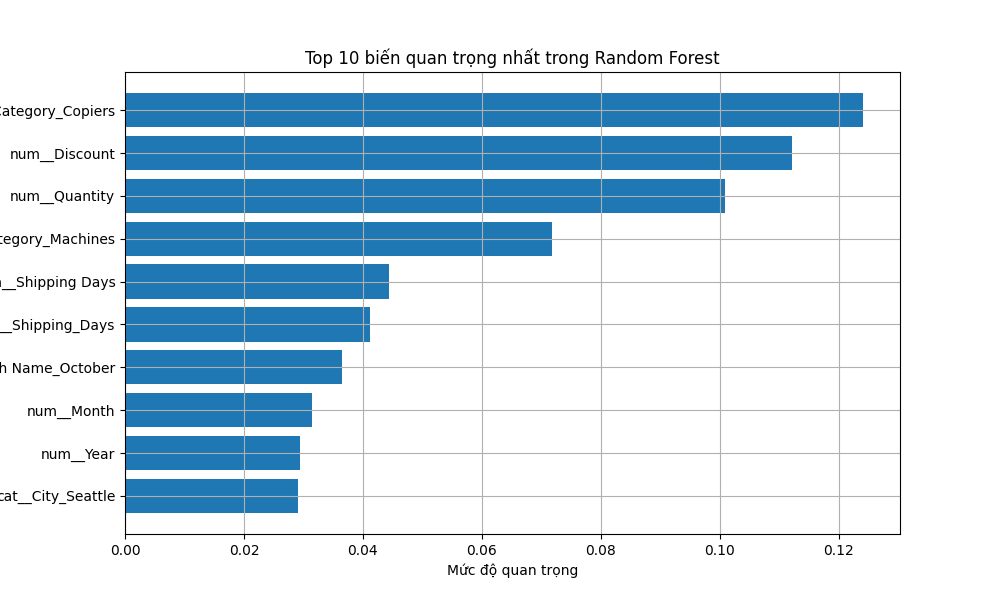
\includegraphics[width=0.8\textwidth]{images/anh_chuong4/random_forest_feature_importance.png}
	\caption{\centering Mức độ quan trọng của các biến trước khi xử lý ngoại lai}
	\label{fig:rf_importance_after_clean}
\end{figure}

Quan sát Hình \ref{fig:rf_importance_after_clean} cho thấy các biến như Discount, Quantity và một số nhóm sản phẩm có ảnh hưởng lớn đến khả năng dự báo lợi nhuận của mô hình.	

\refstepcounter{subsection}
\subsection*{\thesubsection\quad Kết quả sau xử lý ngoại lai}

Sau khi xử lý ngoại lai bằng phương pháp IQR Capping, hiệu quả của mô hình Random Forest được cải thiện rõ rệt trên cả tập huấn luyện và tập kiểm tra.

Cụ thể:
\begin{itemize}
	\item Tập huấn luyện đạt \(MAE = 10.7544\), \(RMSE = 14.7411\) và \(R^2 = 0.7484\).
	\item Tập kiểm tra đạt \(MAE = 15.49\), \(RMSE = 20.9505\) và \(R^2 = 0.4892\).
\end{itemize}

Giá trị \(R^2\) tăng đáng kể so với trước xử lý ngoại lai, đồng thời các chỉ số MAE và RMSE giảm rõ rệt. Điều này cho thấy việc xử lý ngoại lai giúp mô hình học ổn định hơn và cải thiện khả năng dự báo lợi nhuận.

\begin{figure}[H]
	\centering
	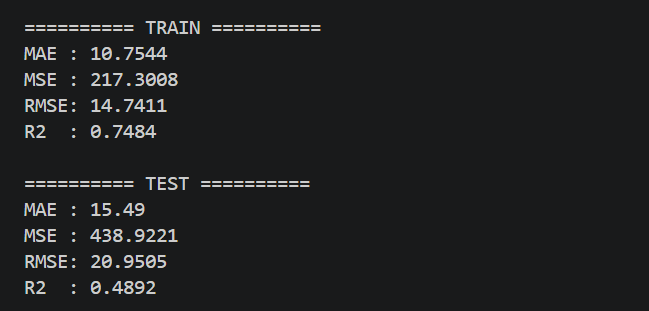
\includegraphics[width=0.6\textwidth]{images/anh_chuong4/random_forest_after_metrics.png}
	\caption{\centering Kết quả mô hình Random Forest sau xử lý ngoại lai}
	\label{fig:rf_after_metrics}
\end{figure}

Nguyên nhân là do các giá trị lợi nhuận quá lớn hoặc quá nhỏ đã được giới hạn trong khoảng hợp lý hơn, giúp các cây quyết định tập trung tốt hơn vào xu hướng chung của dữ liệu thay vì học quá mức từ các giao dịch bất thường.

\begin{figure}[H]
	\centering
	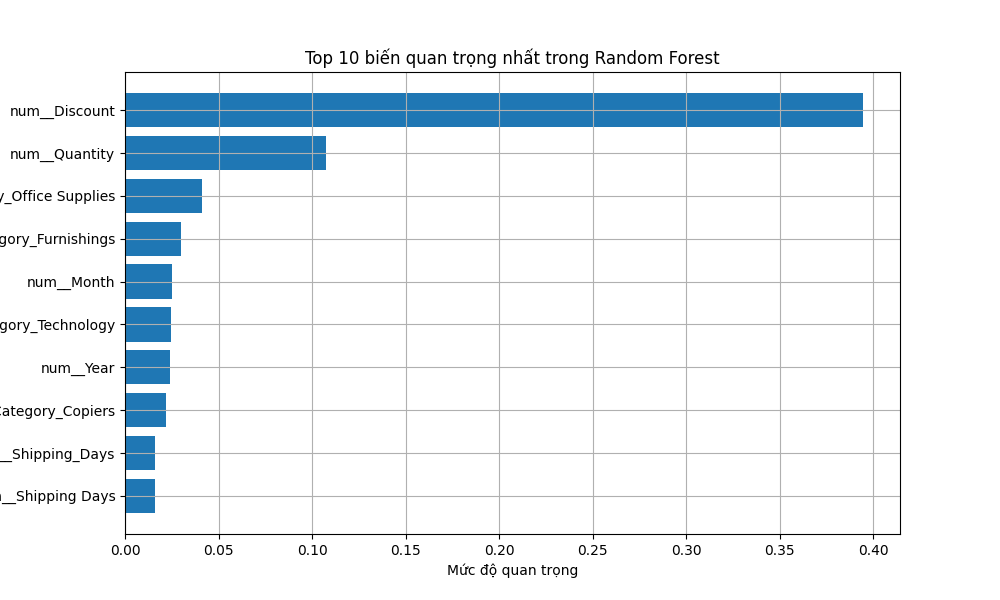
\includegraphics[width=0.8\textwidth]{images/anh_chuong4/random_forest_after_feature_importance.png}
	\caption{\centering Mức độ quan trọng của các biến sau xử lý ngoại lai}
	\label{fig:rf_after_feature_importance}
\end{figure}

Quan sát Hình \ref{fig:rf_after_feature_importance} cho thấy biến Discount có ảnh hưởng lớn nhất đến khả năng dự báo lợi nhuận của mô hình. Ngoài ra, Quantity và một số nhóm sản phẩm cũng có mức độ ảnh hưởng đáng kể, phản ánh lợi nhuận trong dữ liệu bán lẻ chịu tác động mạnh bởi chính sách chiết khấu và đặc điểm sản phẩm.

\refstepcounter{subsection}
\subsection*{\thesubsection\quad So sánh trước và sau xử lý ngoại lai}

Sau khi xử lý ngoại lai, hiệu quả của mô hình Random Forest được cải thiện rõ rệt. Giá trị \(R^2\) trên tập kiểm tra tăng từ 0.1063 lên 0.4892, đồng thời các chỉ số MAE và RMSE giảm đáng kể so với trước xử lý ngoại lai.

Mặc dù Random Forest có khả năng chống chịu ngoại lai tốt hơn hồi quy tuyến tính, việc xử lý ngoại lai vẫn giúp mô hình học ổn định hơn và nâng cao khả năng tổng quát hóa trên tập kiểm tra. Điều này cho thấy việc làm sạch dữ liệu có vai trò quan trọng trong bài toán dự báo lợi nhuận đối với dữ liệu bán lẻ.

\refstepcounter{subsection}
\subsection*{\thesubsection\quad Nhận xét mô hình}

Random Forest là mô hình cho kết quả khá tốt trong bài toán dự báo lợi nhuận nhờ khả năng học được các quan hệ phi tuyến và tương tác giữa nhiều biến đầu vào. Sau khi xử lý ngoại lai, hiệu quả mô hình được cải thiện đáng kể và tốt hơn nhiều so với hồi quy tuyến tính đa biến.

Ngoài ra, Random Forest còn có ưu điểm trong việc xác định mức độ quan trọng của các biến, qua đó hỗ trợ phân tích các yếu tố ảnh hưởng đến lợi nhuận trong dữ liệu bán lẻ.

\section{Mô hình Gradient Boosting}

\refstepcounter{subsection}
\subsection*{\thesubsection\quad Giới thiệu mô hình}

Gradient Boosting Regressor là mô hình thuộc nhóm boosting. Khác với Random Forest xây dựng nhiều cây tương đối độc lập, Gradient Boosting xây dựng các cây theo cách tuần tự. Mỗi cây mới được huấn luyện nhằm giảm phần sai số mà các cây trước đó chưa dự báo tốt.

Cơ chế này giúp Gradient Boosting có khả năng học sâu hơn các quy luật phức tạp trong dữ liệu. Mô hình đặc biệt phù hợp với dữ liệu dạng bảng, nơi biến mục tiêu chịu ảnh hưởng bởi nhiều yếu tố và các mối quan hệ không hoàn toàn tuyến tính.

\refstepcounter{subsection}
\subsection*{\thesubsection\quad Kết quả trước xử lý ngoại lai}

Trước khi xử lý ngoại lai, mô hình Gradient Boosting cho kết quả chưa tốt trên tập kiểm tra với giá trị \(R^2 = -0.033\). Giá trị \(R^2\) âm cho thấy mô hình dự báo kém hơn cả việc sử dụng giá trị trung bình của biến Profit để dự báo.

Cụ thể:
\begin{itemize}
	\item Tập huấn luyện đạt \(MAE = 55.3735\), \(RMSE = 162.5168\) và \(R^2 = 0.575\).
	\item Tập kiểm tra đạt \(MAE = 57.0017\), \(RMSE = 149.3123\) và \(R^2 = -0.033\).
\end{itemize}

Kết quả này cho thấy tồn tại sự chênh lệch lớn giữa tập huấn luyện và tập kiểm tra. Mô hình học khá tốt trên dữ liệu huấn luyện nhưng chưa tổng quát hóa tốt trên dữ liệu kiểm tra khi dữ liệu vẫn chứa nhiều giá trị ngoại lai.

\begin{figure}[H]
	\centering
	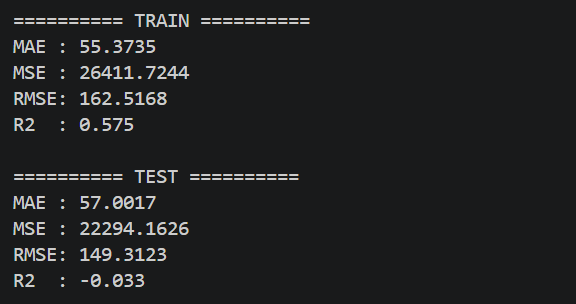
\includegraphics[width=0.6\textwidth]{images/anh_chuong4/gradient_boosting_before_metrics.png}
	\caption{\centering Kết quả mô hình Gradient Boosting trước xử lý ngoại lai}
	\label{fig:gb_before_metrics}
\end{figure}

Nguyên nhân chủ yếu đến từ sự tồn tại của nhiều giá trị ngoại lai trong dữ liệu lợi nhuận. Gradient Boosting là mô hình học tuần tự dựa trên sai số của các bước trước, vì vậy các giao dịch có sai số lớn có thể khiến mô hình tập trung quá mức vào những điểm bất thường.

Điều này làm giảm khả năng học xu hướng chung của dữ liệu và ảnh hưởng đến khả năng tổng quát hóa trên tập kiểm tra.

\begin{figure}[H]
	\centering
	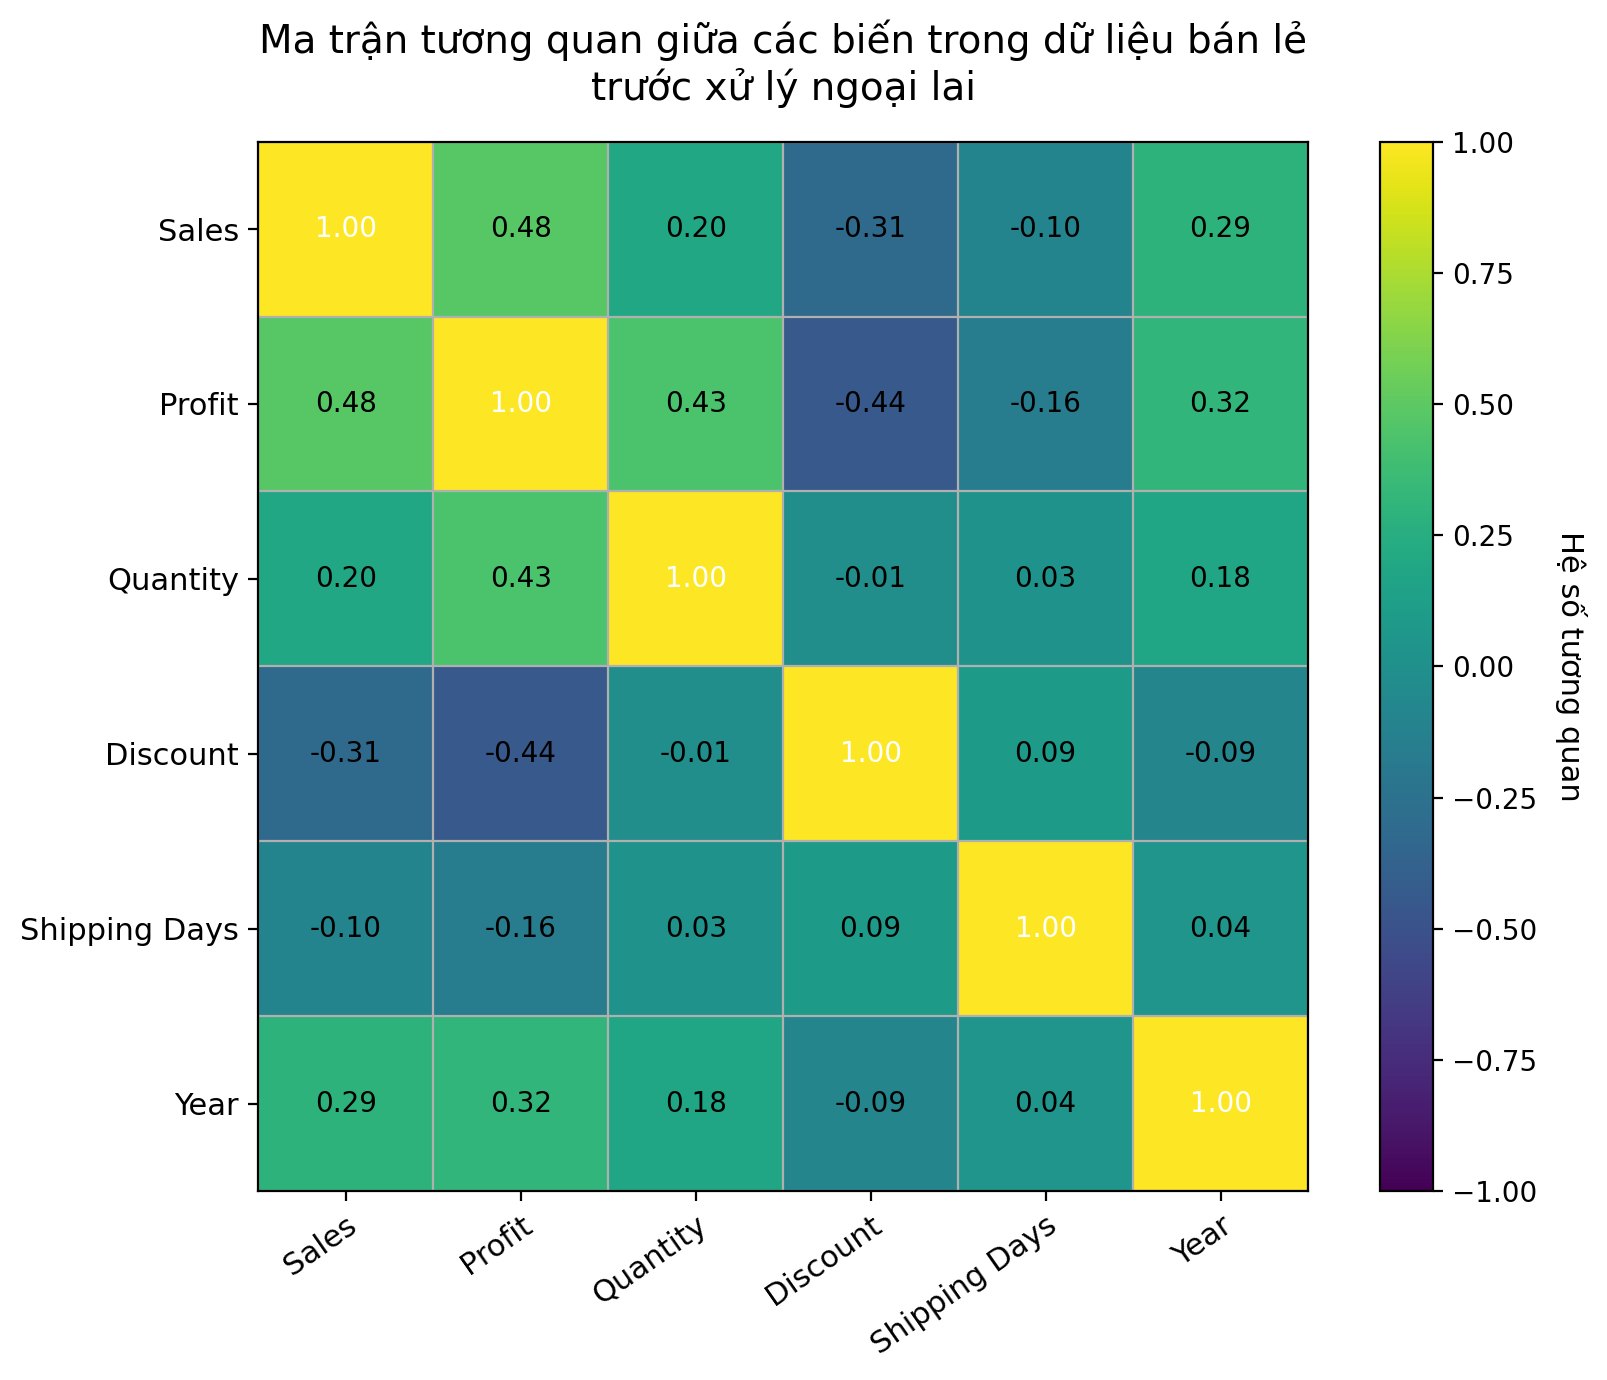
\includegraphics[width=0.8\textwidth]{images/anh_chuong4/Ma_tran_tuong_quan_ban_le.png}
    \caption{\centering Ma trận tương quan giữa các biến số chính trước xử lý ngoại lai}
	\label{fig:gb_before_correlation_matrix}
\end{figure}

Quan sát Hình \ref{fig:gb_before_correlation_matrix} cho thấy các biến trong dữ liệu bán lẻ có mức độ tương quan khác nhau với biến Profit. Trong đó, Discount có tương quan âm với Profit, phản ánh rằng mức chiết khấu cao có thể làm giảm lợi nhuận của doanh nghiệp. Ngược lại, Sales và Quantity có tương quan dương với Profit, cho thấy doanh thu và số lượng bán ra có xu hướng đóng góp tích cực vào lợi nhuận.

Bên cạnh đó, Shipping Days có tương quan yếu với Profit, cho thấy thời gian giao hàng không phải là yếu tố ảnh hưởng mạnh đến lợi nhuận trong bộ dữ liệu này. Biến Year có tương quan dương nhẹ với Profit, phản ánh lợi nhuận có xu hướng cải thiện theo thời gian.

\refstepcounter{subsection}
\subsection*{\thesubsection\quad Kết quả sau xử lý ngoại lai}

Sau khi xử lý ngoại lai bằng phương pháp IQR Capping, hiệu quả của mô hình Gradient Boosting được cải thiện rõ rệt trên cả tập huấn luyện và tập kiểm tra.

Cụ thể:
\begin{itemize}
	\item Tập huấn luyện đạt \(MAE = 15.1713\), \(RMSE = 19.889\) và \(R^2 = 0.542\).
	\item Tập kiểm tra đạt \(MAE = 15.7957\), \(RMSE = 20.652\) và \(R^2 = 0.5036\).
\end{itemize}

Giá trị \(R^2\) trên tập kiểm tra tăng mạnh từ \(-0.033\) lên \(0.5036\), đồng thời các chỉ số MAE và RMSE giảm đáng kể. Điều này cho thấy việc xử lý ngoại lai giúp mô hình học ổn định hơn và nâng cao khả năng dự báo lợi nhuận.

\begin{figure}[H]
	\centering
	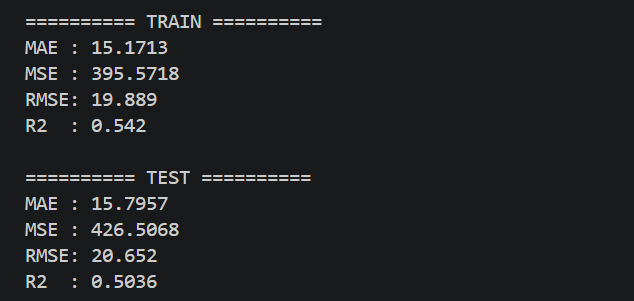
\includegraphics[width=0.6\textwidth]{images/anh_chuong4/gradient_boosting_after_metrics.png}
	\caption{\centering Kết quả mô hình Gradient Boosting sau xử lý ngoại lai}
	\label{fig:gb_after_metrics}
\end{figure}

Nguyên nhân là do các giá trị lợi nhuận bất thường đã được kiểm soát tốt hơn, giúp mô hình không còn tập trung quá mức vào các giao dịch cực đoan. Nhờ đó, Gradient Boosting có thể học hiệu quả hơn các xu hướng chung trong dữ liệu bán lẻ.

Ngoài ra, kết quả của Gradient Boosting sau xử lý ngoại lai cũng cao hơn Random Forest trên tập kiểm tra. Điều này cho thấy cơ chế học tuần tự của boosting có khả năng khai thác tốt các quan hệ phức tạp giữa các biến khi dữ liệu đầu vào được xử lý phù hợp.

\begin{figure}[H]
	\centering
	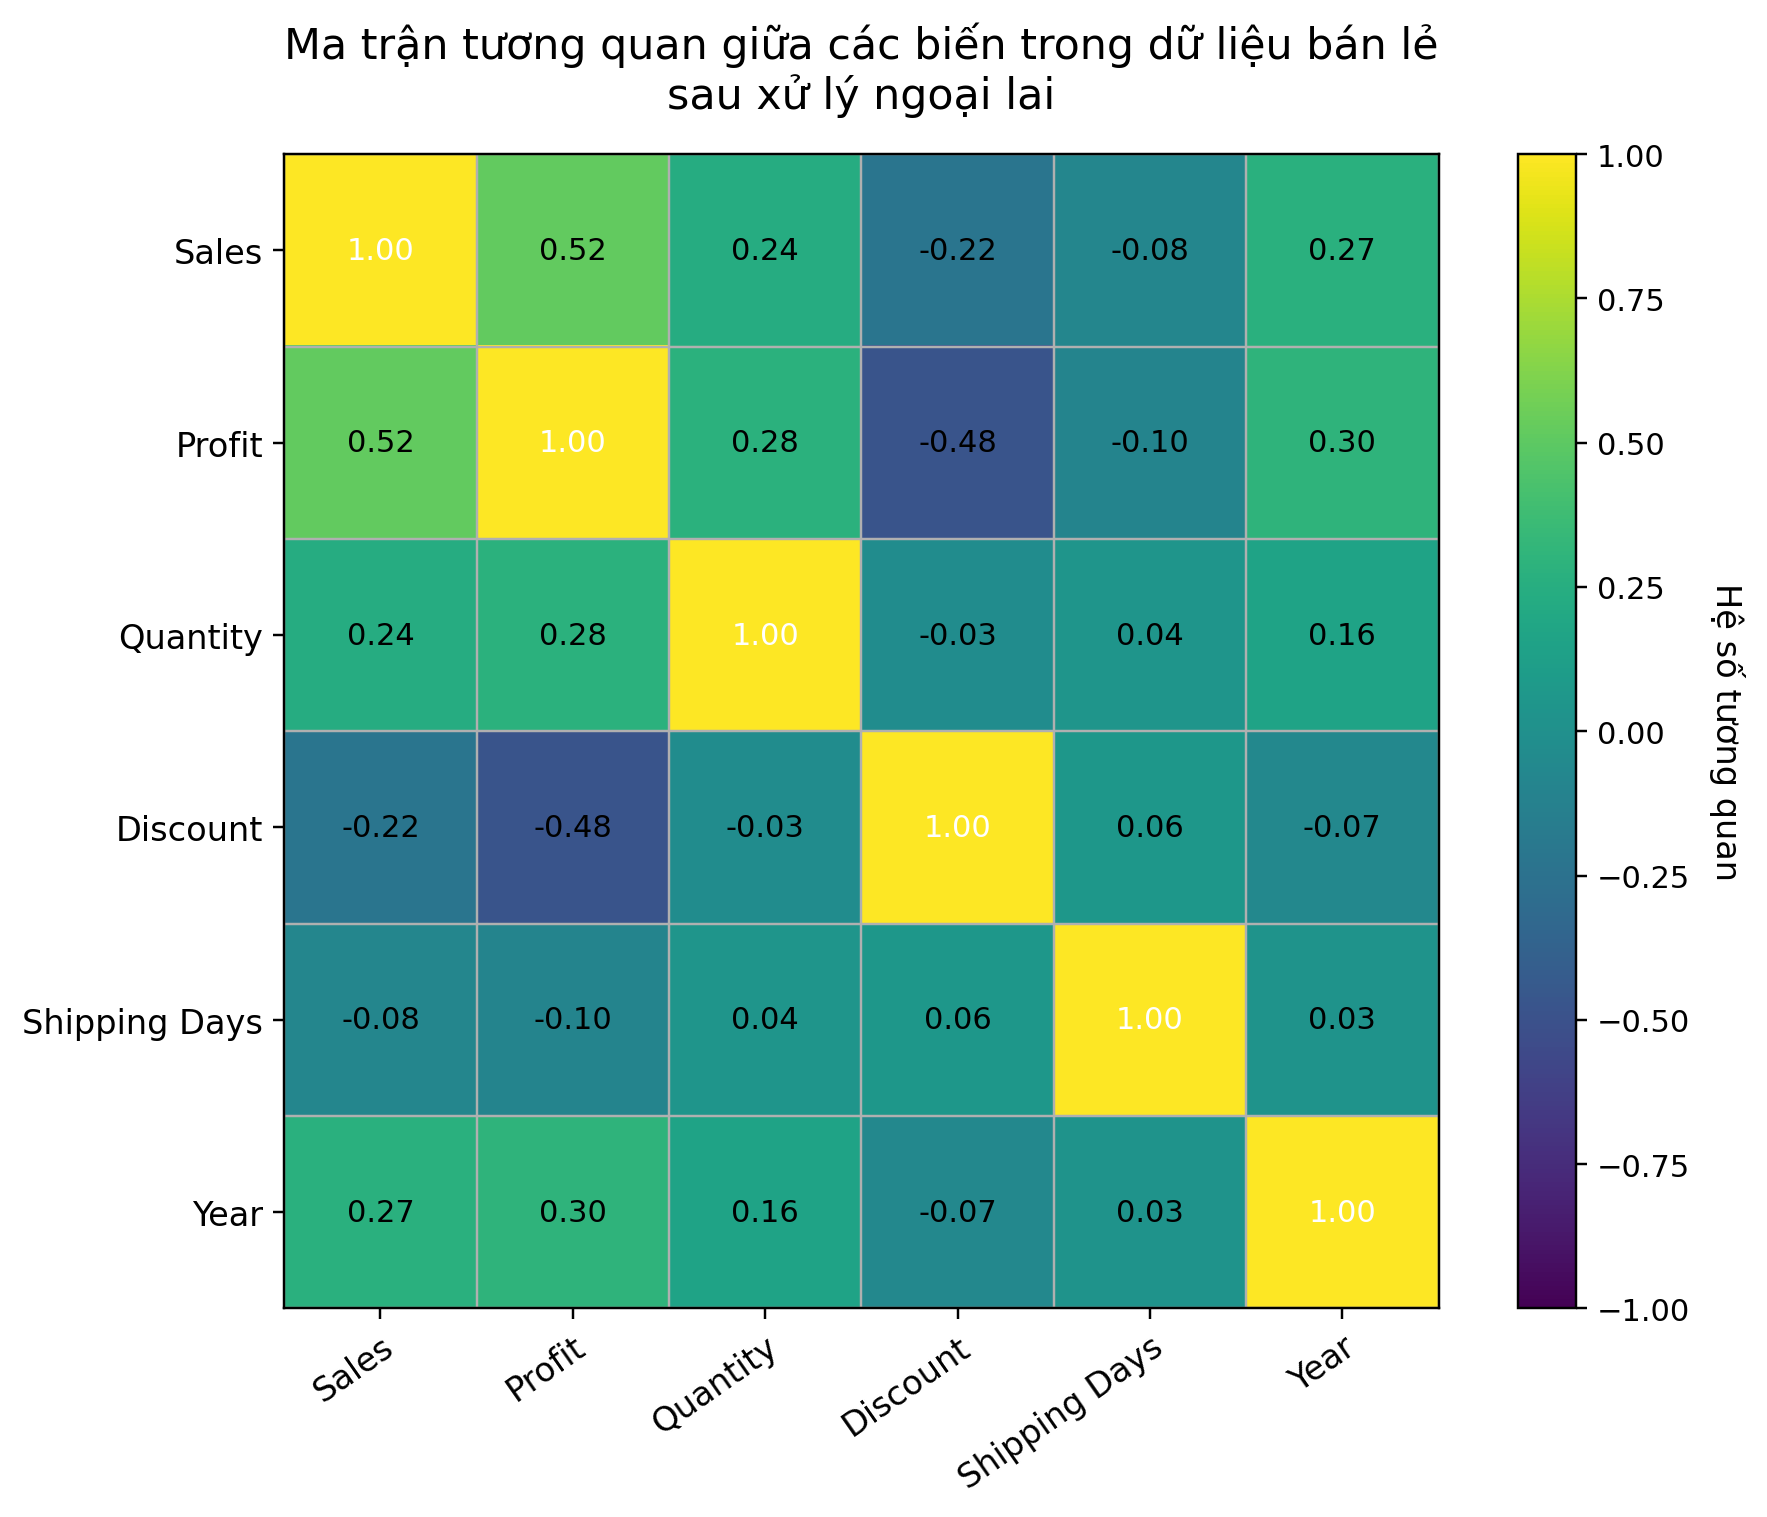
\includegraphics[width=0.85\textwidth]{images/anh_chuong4/Ma_tran_tuong_quan_sau_xu_ly_ngoai_lai.png}
    \caption{\centering Ma trận tương quan giữa các biến số chính sau xử lý ngoại lai}
	\label{fig:gb_after_correlation_matrix}
\end{figure}

Quan sát Hình \ref{fig:gb_after_correlation_matrix} cho thấy các biến trong dữ liệu bán lẻ vẫn có mức độ tương quan khác nhau với biến Profit sau khi xử lý ngoại lai. Trong đó, Discount tiếp tục có tương quan âm với Profit, phản ánh rằng mức chiết khấu cao vẫn có xu hướng làm giảm lợi nhuận của doanh nghiệp. Ngược lại, Sales và Quantity có tương quan dương với Profit, cho thấy doanh thu và số lượng bán ra vẫn là những yếu tố đóng góp tích cực vào lợi nhuận.

Ngoài ra, Shipping Days có tương quan yếu với Profit, cho thấy thời gian giao hàng không phải là yếu tố ảnh hưởng mạnh đến lợi nhuận trong bộ dữ liệu này. Biến Year có tương quan dương nhẹ với Profit, phản ánh lợi nhuận có xu hướng cải thiện theo thời gian sau khi dữ liệu đã được làm sạch.


\refstepcounter{subsection}
\subsection*{\thesubsection\quad So sánh trước và sau xử lý ngoại lai}

Gradient Boosting là mô hình có sự cải thiện rõ rệt sau khi xử lý ngoại lai. Giá trị \(R^2\) trên tập kiểm tra tăng từ \(-0.033\) lên \(0.5036\), đồng thời MAE và RMSE giảm đáng kể.

Kết quả này cho thấy mô hình boosting khá nhạy cảm với các giá trị ngoại lai trong dữ liệu. Khi dữ liệu chưa được xử lý, mô hình dễ tập trung quá mức vào các giao dịch bất thường. Sau khi làm sạch dữ liệu, Gradient Boosting học ổn định hơn và khai thác tốt các quan hệ phi tuyến giữa các biến, từ đó nâng cao hiệu quả dự báo.

\refstepcounter{subsection}
\subsection*{\thesubsection\quad Nhận xét mô hình}

Gradient Boosting cho kết quả tốt sau khi xử lý ngoại lai và có khả năng tổng quát hóa tương đối ổn định trên tập kiểm tra. Mô hình phù hợp với bài toán dự báo lợi nhuận nhờ khả năng học được các quan hệ phi tuyến và tương tác phức tạp giữa nhiều biến đầu vào.

Tuy nhiên, mô hình khá nhạy cảm với các giá trị ngoại lai do cơ chế học tuần tự dựa trên sai số. Nếu dữ liệu chứa nhiều điểm bất thường, mô hình có thể tập trung quá mức vào các giao dịch ngoại lệ và làm giảm hiệu quả dự báo. Vì vậy, bước xử lý ngoại lai đóng vai trò quan trọng trong việc nâng cao hiệu quả của Gradient Boosting trong đề tài này.

\section{Mô hình XGBoost}

\refstepcounter{subsection}
\subsection*{\thesubsection\quad Giới thiệu mô hình}

XGBoost Regressor là mô hình boosting nâng cao, được phát triển nhằm cải thiện hiệu quả dự báo và tốc độ huấn luyện. Mô hình vẫn dựa trên nguyên lý xây dựng các cây quyết định theo cách tuần tự, nhưng bổ sung thêm cơ chế để kiểm soát độ phức tạp của mô hình và hạn chế hiện tượng quá khớp.

XGBoost thường cho kết quả tốt đối với dữ liệu dạng bảng, đặc biệt trong các bài toán dự báo có nhiều biến định tính sau khi mã hóa. Sau khi được mã hóa bằng One-Hot Encoding, các biến này tạo thành tập đặc trưng dạng bảng phù hợp với XGBoost.

\refstepcounter{subsection}
\subsection*{\thesubsection\quad Kết quả trước xử lý ngoại lai}

Trước khi xử lý ngoại lai, mô hình XGBoost cho kết quả tốt hơn hồi quy tuyến tính đa biến và Gradient Boosting trên tập kiểm tra với giá trị \(R^2 = 0.1204\). Điều này cho thấy XGBoost có khả năng học dữ liệu tốt hơn ngay cả khi dữ liệu còn chứa nhiều nhiễu và giá trị bất thường.

Cụ thể:
\begin{itemize}
	\item Tập huấn luyện đạt \(MAE = 49.3776\), \(RMSE = 124.2613\) và \(R^2 = 0.7515\).
	\item Tập kiểm tra đạt \(MAE = 54.7294\), \(RMSE = 137.7825\) và \(R^2 = 0.1204\).
\end{itemize}

Mặc dù kết quả trên tập train khá cao, hiệu quả trên tập test vẫn còn thấp. Điều này cho thấy mô hình có dấu hiệu overfitting và vẫn chịu ảnh hưởng bởi các giá trị ngoại lai trong dữ liệu lợi nhuận.

\begin{figure}[H]
	\centering
	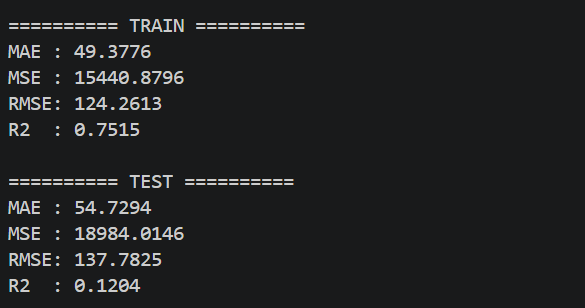
\includegraphics[width=0.6\textwidth]{images/anh_chuong4/xgboost_before_metrics.png}
	\caption{\centering Kết quả mô hình XGBoost trước xử lý ngoại lai}
	\label{fig:xgb_before_metrics}
\end{figure}

Nguyên nhân chủ yếu đến từ các giao dịch có lợi nhuận quá lớn hoặc quá nhỏ làm tăng độ biến động của biến Profit. Các giá trị ngoại lai khiến mô hình khó học chính xác xu hướng chung của dữ liệu và làm giảm khả năng tổng quát hóa trên tập kiểm tra.

Mặc dù XGBoost có cơ chế regularization giúp hạn chế overfitting tốt hơn nhiều mô hình khác, mô hình vẫn không thể loại bỏ hoàn toàn ảnh hưởng của dữ liệu bất thường nếu ngoại lai xuất hiện với mức độ lớn.

\begin{figure}[H]
	\centering
	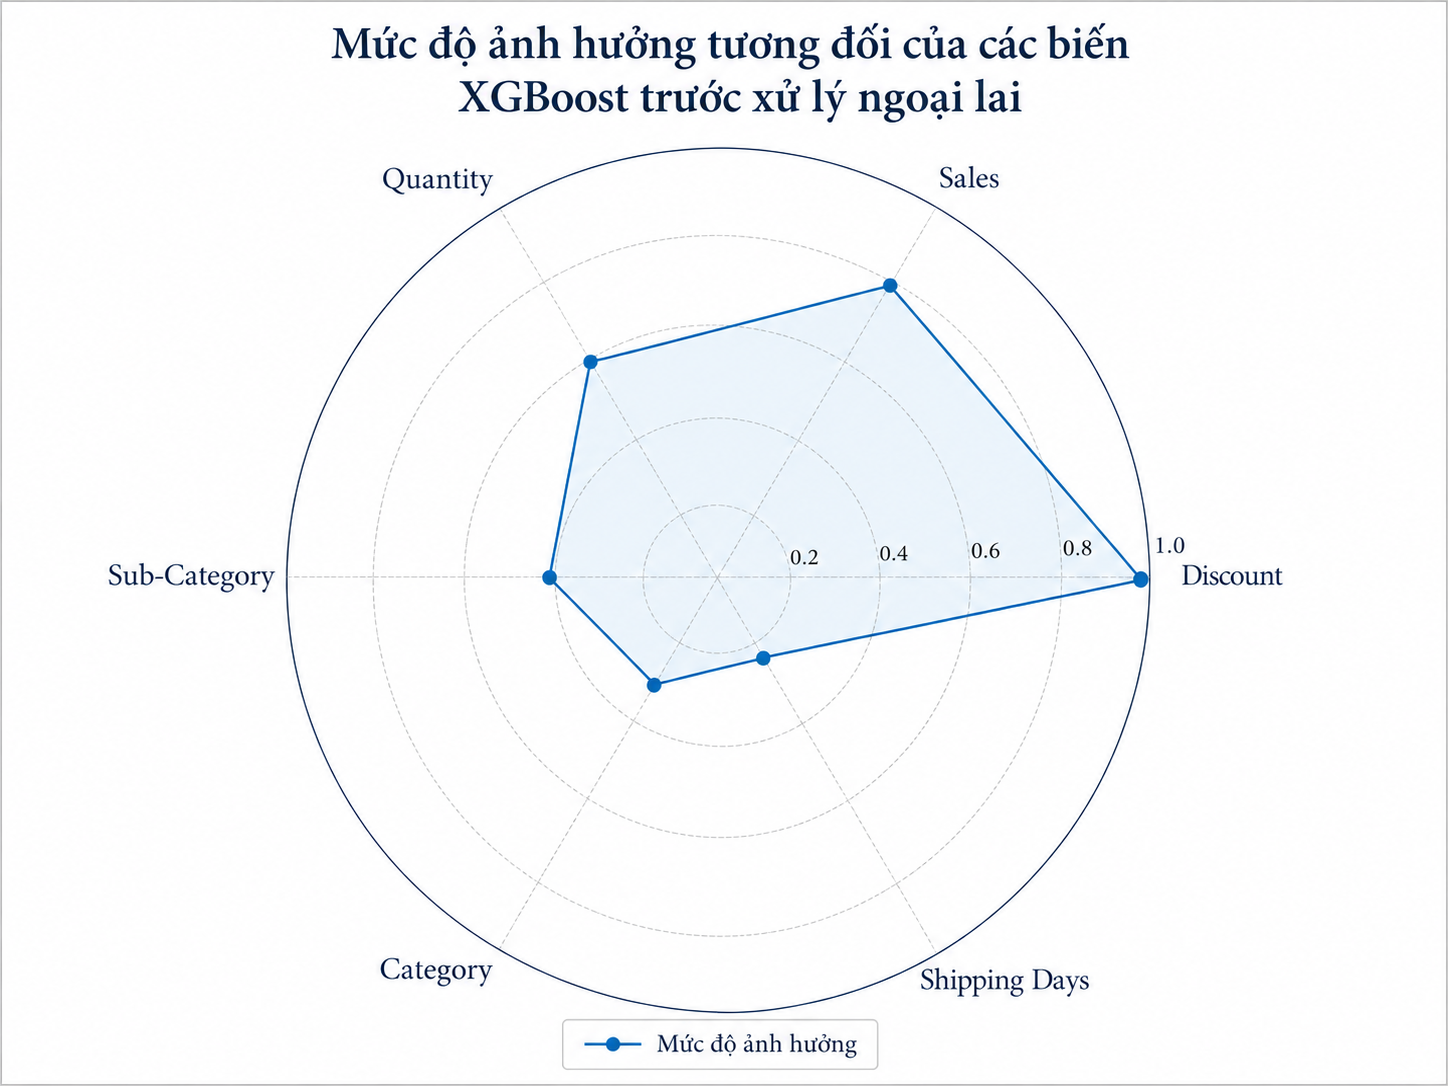
\includegraphics[width=0.8\textwidth]{images/anh_chuong4/1.png}
	\caption{\centering Mức độ ảnh hưởng của các biến trước xử lý ngoại lai}
	\label{fig:xgb_before_radar_importance}
\end{figure}

Quan sát Hình \ref{fig:xgb_before_radar_importance} cho thấy Discount là biến có mức độ ảnh hưởng lớn nhất trong mô hình XGBoost trước xử lý ngoại lai. Điều này cho thấy chính sách chiết khấu có vai trò quan trọng trong việc dự báo lợi nhuận của doanh nghiệp.

Bên cạnh đó, Sales và Quantity cũng có mức độ ảnh hưởng tương đối cao, phản ánh rằng doanh thu và số lượng bán ra là các yếu tố liên quan trực tiếp đến lợi nhuận. Các biến như Sub-Category, Category và Shipping Days có mức độ ảnh hưởng thấp hơn, nhưng vẫn góp phần bổ sung thông tin cho mô hình trong quá trình dự báo.

\refstepcounter{subsection}
\subsection*{\thesubsection\quad Kết quả sau xử lý ngoại lai}

Sau khi xử lý ngoại lai, mô hình XGBoost cho kết quả tốt nhất trong các mô hình dự báo lợi nhuận. Giá trị \(R^2\) trên tập kiểm tra tăng đáng kể lên khoảng 0.5109, đồng thời các chỉ số MAE và RMSE giảm rõ rệt.

Cụ thể:
\begin{itemize}
	\item Tập huấn luyện đạt \(MAE = 14.4558\), \(RMSE = 19.0851\) và \(R^2 = 0.5782\).
	\item Tập kiểm tra đạt \(MAE = 15.5767\), \(RMSE = 20.5\) và \(R^2 = 0.5109\).
\end{itemize}

Kết quả này cho thấy XGBoost có khả năng học hiệu quả các quan hệ phi tuyến và các tương tác phức tạp giữa nhiều biến trong dữ liệu bán lẻ.

\begin{figure}[H]
	\centering
	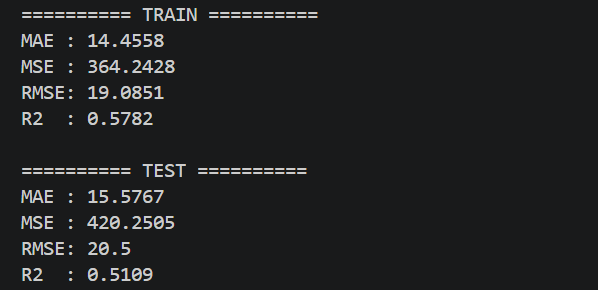
\includegraphics[width=0.6\textwidth]{images/anh_chuong4/xgboost_after_metrics.png}
	\caption{\centering Kết quả mô hình XGBoost sau xử lý ngoại lai}
	\label{fig:xgb_after_metrics}
\end{figure}

Sau khi các giá trị ngoại lai được kiểm soát, mô hình không còn bị ảnh hưởng quá mạnh bởi các giao dịch cực đoan. Điều này giúp quá trình học diễn ra ổn định hơn và nâng cao khả năng tổng quát hóa trên tập kiểm tra.

Ngoài ra, XGBoost cũng cho kết quả tốt hơn Random Forest và Gradient Boosting sau xử lý ngoại lai. Điều này cho thấy cơ chế boosting kết hợp regularization của XGBoost phù hợp với dữ liệu bán lẻ và có khả năng khai thác tốt các đặc trưng quan trọng trong dữ liệu.

\begin{figure}[H]
	\centering
	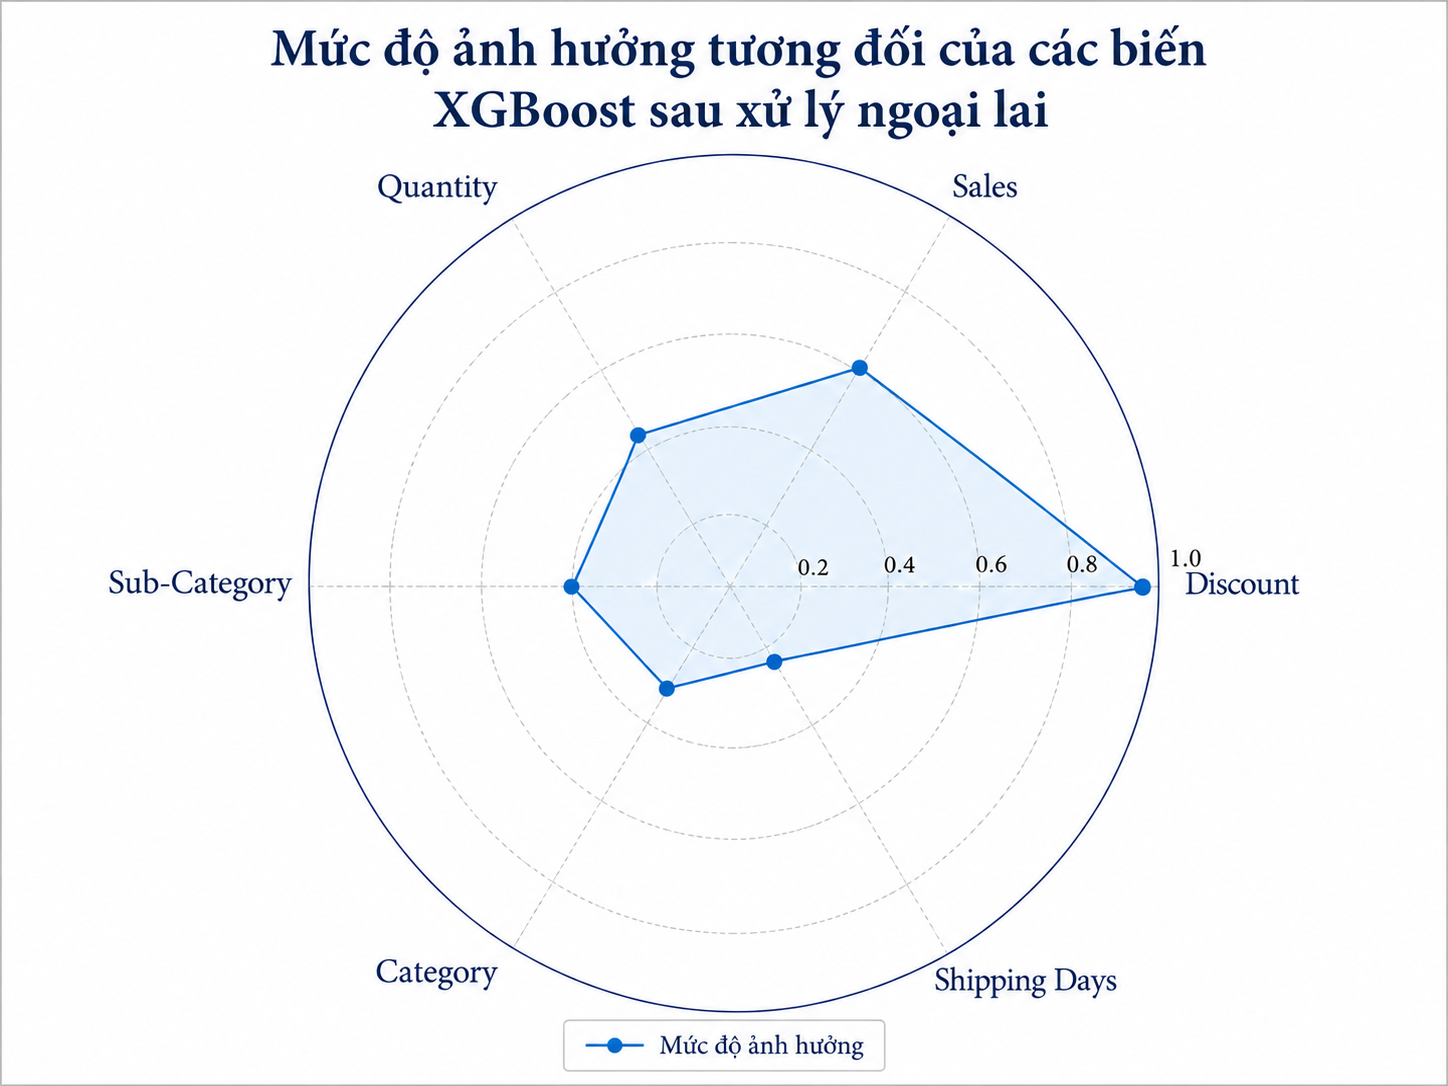
\includegraphics[width=0.8\textwidth]{images/anh_chuong4/2.png}
    \caption{\centering Mức độ ảnh hưởng của các biến sau xử lý ngoại lai}
	\label{fig:xgb_after_importance}
\end{figure}

Quan sát Hình \ref{fig:xgb_after_importance} cho thấy Discount tiếp tục là biến có mức độ ảnh hưởng lớn nhất đến khả năng dự báo lợi nhuận của mô hình XGBoost sau khi xử lý ngoại lai. Bên cạnh đó, một số biến thuộc nhóm sản phẩm và khu vực cũng có vai trò đáng kể trong quá trình dự báo. Kết quả này cho thấy lợi nhuận trong dữ liệu bán lẻ không chỉ chịu tác động mạnh bởi chính sách chiết khấu mà còn phụ thuộc vào đặc điểm sản phẩm và yếu tố thị trường ở từng khu vực.

\refstepcounter{subsection}
\subsection*{\thesubsection\quad So sánh trước và sau xử lý ngoại lai}

Sau khi xử lý ngoại lai, hiệu quả của mô hình XGBoost được cải thiện rõ rệt. Giá trị \(R^2\) trên tập kiểm tra tăng từ 0.1204 lên 0.5109, đồng thời các chỉ số MAE và RMSE giảm đáng kể so với trước xử lý ngoại lai.

Mặc dù XGBoost vốn đã có khả năng xử lý dữ liệu phức tạp và hạn chế overfitting khá tốt, các giá trị ngoại lai vẫn ảnh hưởng đáng kể đến khả năng dự báo của mô hình. Sau khi dữ liệu được làm sạch, mô hình học ổn định hơn và nâng cao khả năng tổng quát hóa trên tập kiểm tra.

Kết quả này cho thấy xử lý ngoại lai là bước quan trọng giúp XGBoost phát huy tốt hơn hiệu quả dự báo trong bài toán dữ liệu bán lẻ.

\refstepcounter{subsection}
\subsection*{\thesubsection\quad Nhận xét mô hình}

XGBoost là mô hình cho kết quả tốt nhất trong bài toán dự báo lợi nhuận của đề tài. Mô hình đạt giá trị \(R^2\) cao nhất trên tập kiểm tra và có các chỉ số sai số thấp hơn so với các mô hình còn lại.

Ưu điểm của XGBoost nằm ở khả năng học các quan hệ phi tuyến, xử lý hiệu quả dữ liệu dạng bảng và kiểm soát độ phức tạp của mô hình thông qua cơ chế regularization. Điều này giúp mô hình phù hợp với dữ liệu bán lẻ vốn có nhiều mối quan hệ và tương tác phức tạp giữa các biến.

Từ kết quả thực nghiệm, có thể thấy XGBoost là mô hình phù hợp nhất trong phạm vi dữ liệu và phương pháp triển khai của đề tài.


\section{Mô hình K-Means Clustering}

\refstepcounter{subsection}
\subsection*{\thesubsection\quad Giới thiệu mô hình}

K-Means Clustering là mô hình học không giám sát được sử dụng để phân nhóm các đối tượng dựa trên mức độ tương đồng giữa chúng. Khác với các mô hình hồi quy, K-Means không sử dụng biến mục tiêu mà tập trung vào việc tìm ra các nhóm dữ liệu có đặc điểm gần giống nhau.

Trong đề tài, K-Means được sử dụng để phân cụm khách hàng theo đặc điểm tiêu dùng. Dữ liệu được tổng hợp theo từng khách hàng, sau đó xây dựng các biến đặc trưng như tổng doanh thu, tổng lợi nhuận, tổng số lượng mua, số đơn hàng, doanh thu trung bình mỗi đơn, lợi nhuận trung bình mỗi đơn và tỷ suất lợi nhuận.

Các biến sử dụng cho phân cụm gồm:
\begin{itemize}
    \item Total Sales
    \item Total Profit
    \item Total Quantity
    \item Avg Discount
    \item Avg Shipping Days
    \item Order Count
    \item Sales Per Order
    \item Profit Per Order
    \item Profit Margin
\end{itemize}

Trước khi phân cụm, dữ liệu được chuẩn hóa bằng StandardScaler. Đây là bước cần thiết vì các biến có đơn vị đo khác nhau. Nếu không chuẩn hóa, các biến có giá trị lớn như Total Sales hoặc Total Profit có thể chi phối toàn bộ quá trình phân cụm.

\refstepcounter{subsection}
\subsection*{\thesubsection\quad Kết quả trước xử lý ngoại lai}

Trước khi xử lý ngoại lai, dữ liệu khách hàng vẫn tồn tại một số quan sát có tổng doanh thu hoặc tổng lợi nhuận rất lớn so với phần còn lại. Do K-Means sử dụng khoảng cách Euclid để phân nhóm, các giá trị bất thường này có thể làm lệch vị trí tâm cụm và ảnh hưởng đến chất lượng phân cụm.

Kết quả đánh giá số cụm cho thấy tại \(K = 2\), mô hình đạt Silhouette Score khoảng 0.2602. Đây là giá trị cao nhất trong các số cụm được thử nghiệm, vì vậy đề tài lựa chọn \(K = 2\) để thực hiện phân cụm khách hàng trước xử lý ngoại lai.

\begin{figure}[H]
	\centering
	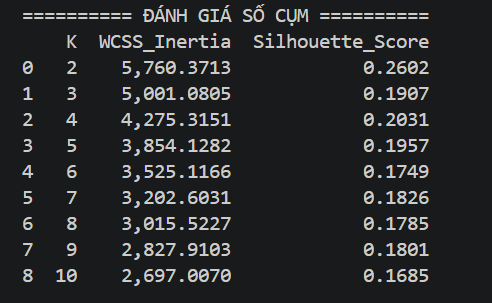
\includegraphics[width=0.6\textwidth]{images/anh_chuong4/kmeans_before_metrics.png}
	\caption{\centering Kết quả đánh giá số cụm K-Means trước xử lý ngoại lai}
	\label{fig:kmeans_before_metrics}
\end{figure}

\begin{figure}[H]
	\centering
	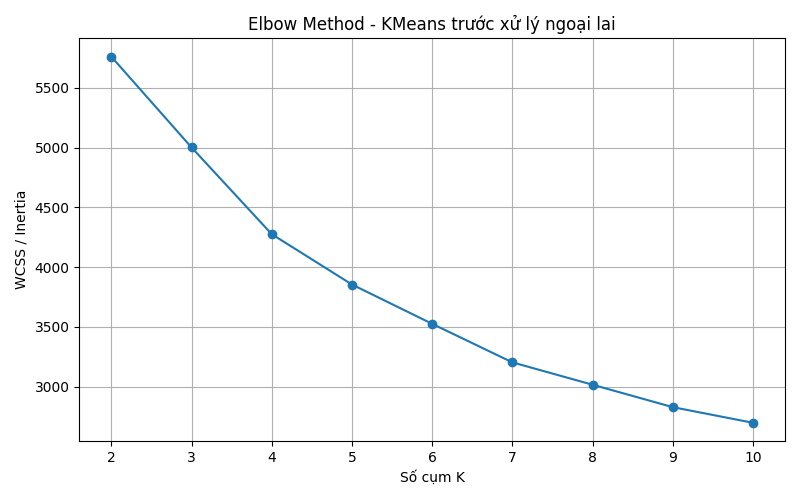
\includegraphics[width=0.7\textwidth]{images/anh_chuong4/kmeans_before_elbow.png}
	\caption{\centering Elbow Method của mô hình K-Means trước xử lý ngoại lai}
	\label{fig:kmeans_before_elbow}
\end{figure}

\begin{figure}[H]
	\centering
	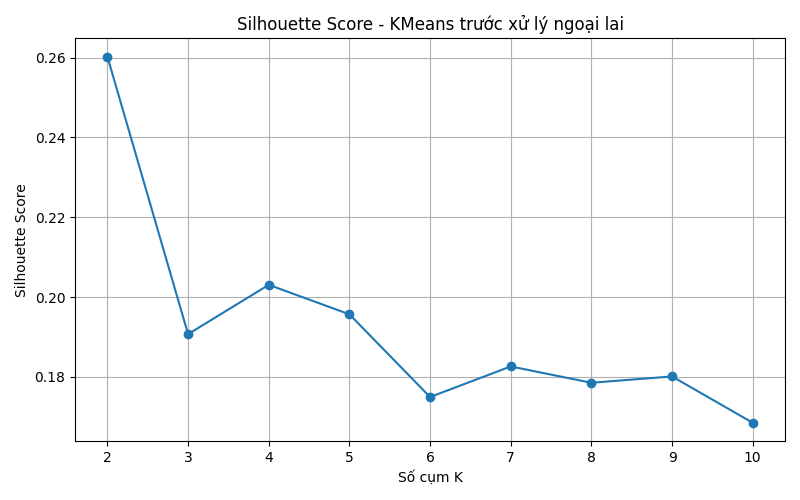
\includegraphics[width=0.7\textwidth]{images/anh_chuong4/kmeans_before_silhouette.png}
	\caption{\centering Silhouette Score của mô hình K-Means trước xử lý ngoại lai}
	\label{fig:kmeans_before_silhouette}
\end{figure}

Quan sát Hình \ref{fig:kmeans_before_elbow} và Hình \ref{fig:kmeans_before_silhouette} cho thấy WCSS giảm dần khi số cụm tăng, trong khi Silhouette Score đạt giá trị cao nhất tại \(K = 2\). Vì vậy, số cụm \(K = 2\) được lựa chọn để phân nhóm khách hàng.

\begin{figure}[H]
	\centering
	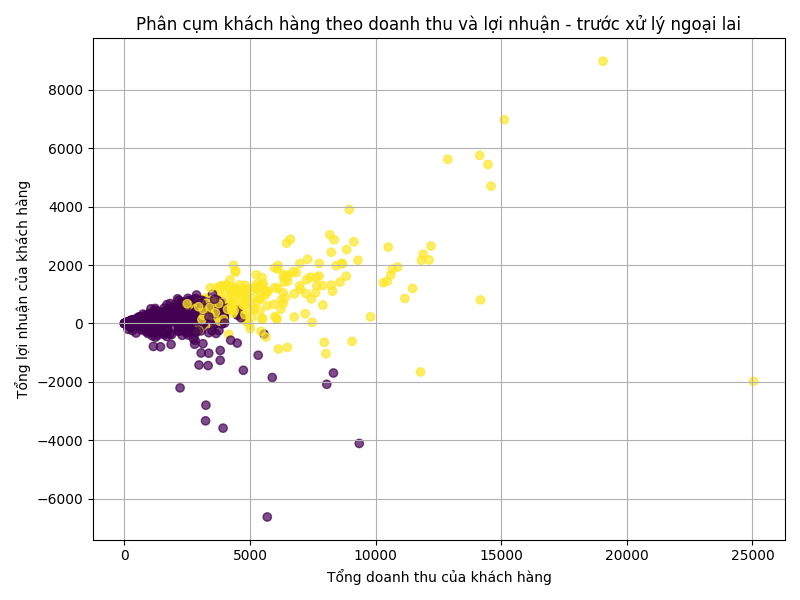
\includegraphics[width=0.8\textwidth]{images/anh_chuong4/kmeans_before_cluster.png}
	\caption{\centering Phân cụm khách hàng trước xử lý ngoại lai}
	\label{fig:kmeans_before_cluster}
\end{figure}

Quan sát Hình \ref{fig:kmeans_before_cluster} cho thấy một số khách hàng có doanh thu hoặc lợi nhuận rất lớn nằm cách xa phần lớn dữ liệu. Các điểm này có thể kéo tâm cụm lệch khỏi vị trí đại diện cho nhóm khách hàng phổ biến, làm giảm tính ổn định của mô hình phân cụm.

\begin{figure}[H]
	\centering
	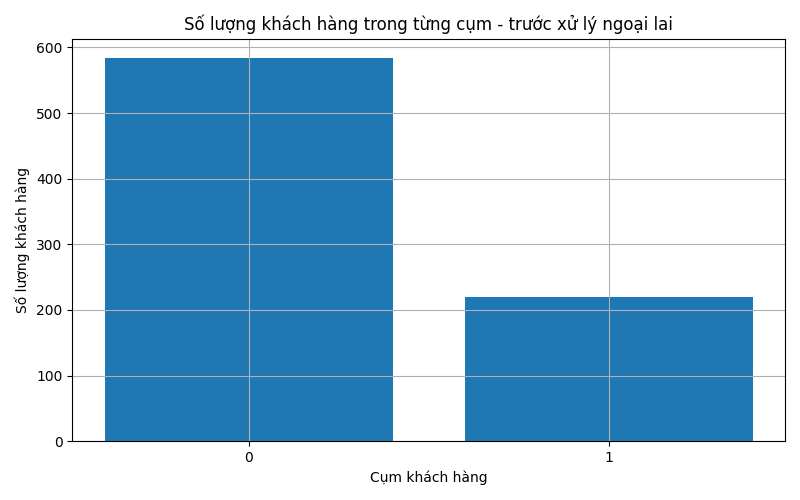
\includegraphics[width=0.65\textwidth]{images/anh_chuong4/kmeans_before_cluster_count.png}
	\caption{\centering Số lượng khách hàng trong từng cụm trước xử lý ngoại lai}
	\label{fig:kmeans_before_cluster_count}
\end{figure}

Biểu đồ số lượng khách hàng cho thấy hai cụm có quy mô không đồng đều. Cụm 0 chiếm phần lớn số lượng khách hàng, trong khi cụm 1 có số lượng ít hơn nhưng thường đại diện cho nhóm khách hàng có giá trị giao dịch cao hơn.

\begin{figure}[H]
	\centering
	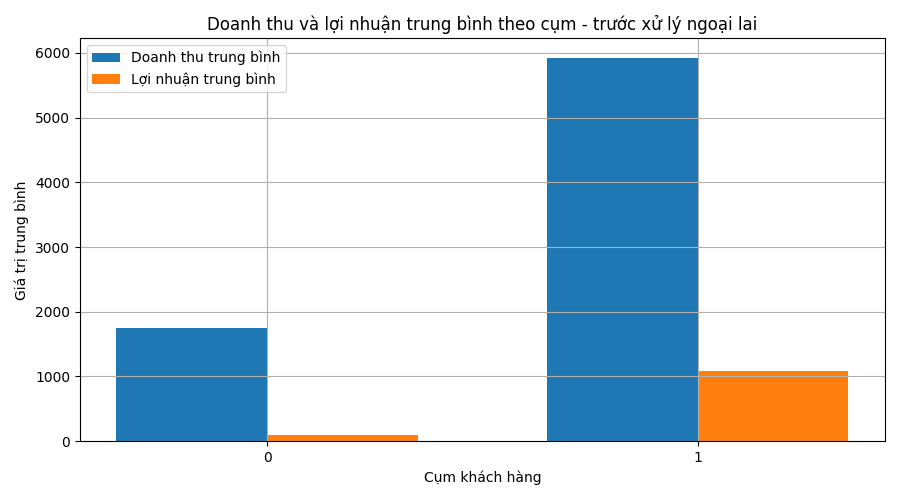
\includegraphics[width=0.75\textwidth]{images/anh_chuong4/kmeans_before_cluster_mean.png}
	\caption{\centering Doanh thu, lợi nhuận trung bình theo cụm trước xử lý ngoại lai}
	\label{fig:kmeans_before_cluster_mean}
\end{figure}

Kết quả doanh thu và lợi nhuận trung bình theo cụm cho thấy cụm 1 có giá trị trung bình cao hơn rõ rệt so với cụm 0. Tuy nhiên, do dữ liệu vẫn còn ngoại lai, kết quả phân cụm có thể bị ảnh hưởng bởi một số khách hàng có doanh thu hoặc lợi nhuận bất thường.

Nhìn chung, trước khi xử lý ngoại lai, K-Means vẫn có thể phân cụm khách hàng thành các nhóm khác nhau. Tuy nhiên, mức độ tách biệt giữa các cụm chưa cao và kết quả còn chịu ảnh hưởng bởi các giá trị cực đoan trong dữ liệu.

\refstepcounter{subsection}
\subsection*{\thesubsection\quad Kết quả sau xử lý ngoại lai}

Sau khi xử lý ngoại lai, dữ liệu khách hàng trở nên ổn định hơn do các giá trị doanh thu và lợi nhuận quá lớn hoặc quá nhỏ đã được giới hạn trong khoảng hợp lý. Điều này giúp mô hình K-Means giảm ảnh hưởng của các điểm cực đoan và xác định tâm cụm chính xác hơn.

Kết quả đánh giá số cụm sau xử lý ngoại lai cho thấy Silhouette Score đạt giá trị cao nhất tại \(K = 2\), với giá trị khoảng 0.2684. Vì vậy, đề tài lựa chọn \(K = 2\) để thực hiện phân cụm khách hàng sau xử lý ngoại lai.

\begin{figure}[H]
	\centering
	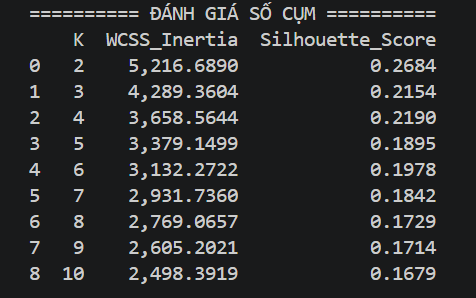
\includegraphics[width=0.6\textwidth]{images/anh_chuong4/kmeans_after_metrics.png}
	\caption{\centering Kết quả đánh giá số cụm K-Means sau xử lý ngoại lai}
	\label{fig:kmeans_after_metrics}
\end{figure}

\begin{figure}[H]
	\centering
	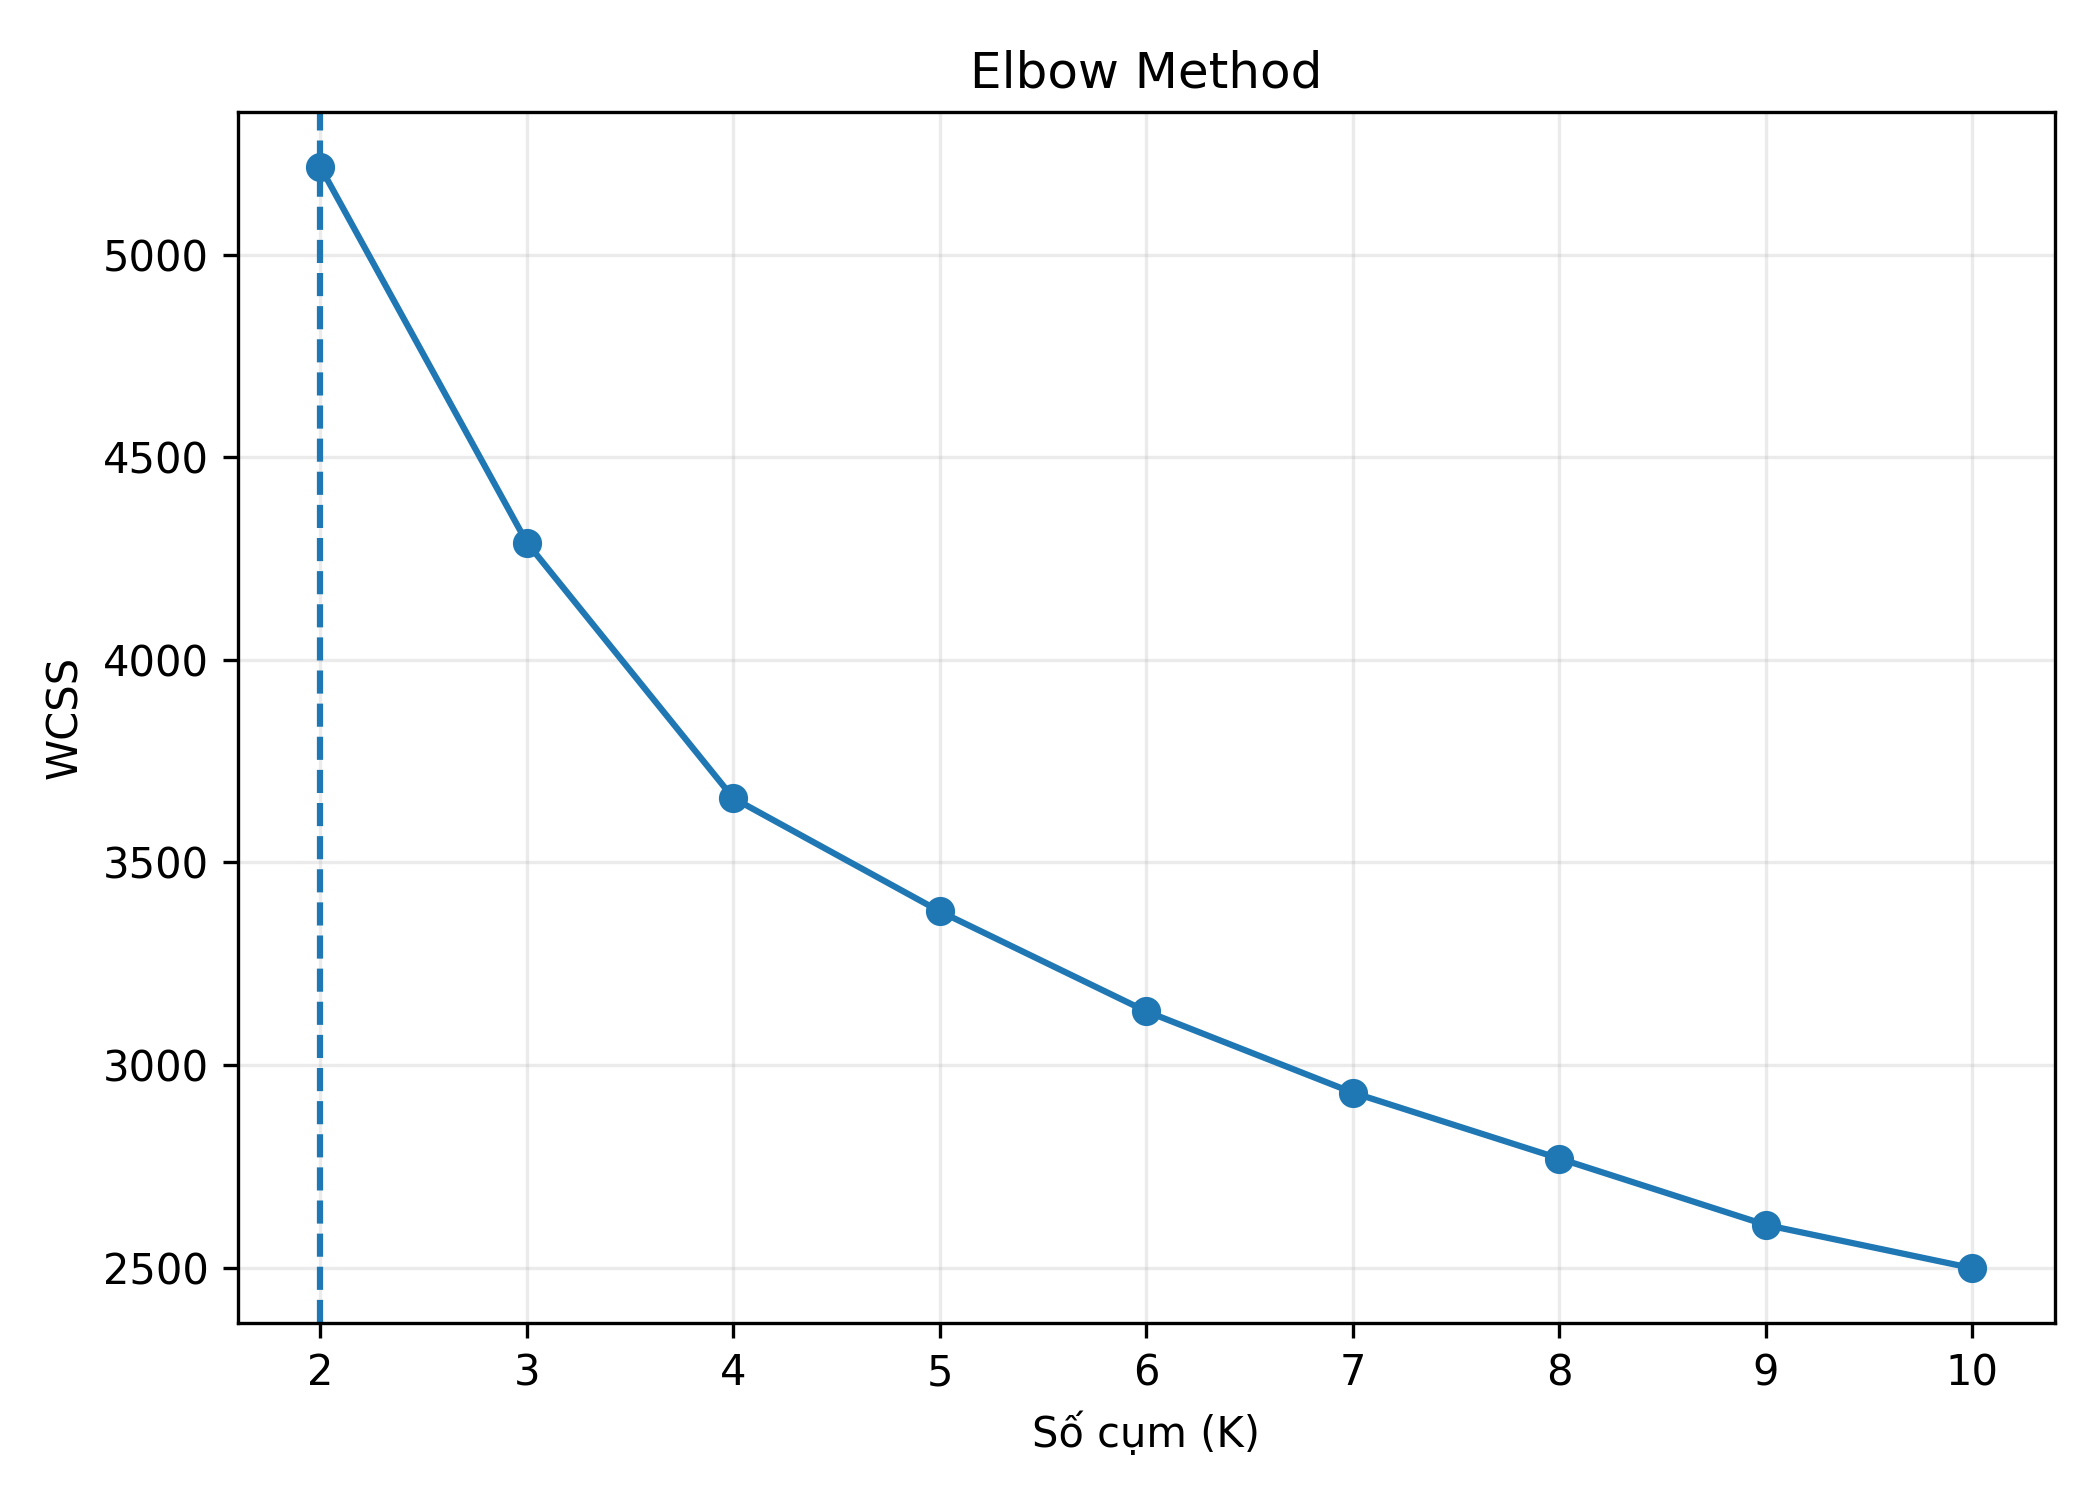
\includegraphics[width=0.7\textwidth]{images/anh_chuong4/kmeans_after_elbow.png}
	\caption{\centering Elbow Method của mô hình K-Means sau xử lý ngoại lai}
	\label{fig:kmeans_after_elbow}
\end{figure}

\begin{figure}[H]
	\centering
	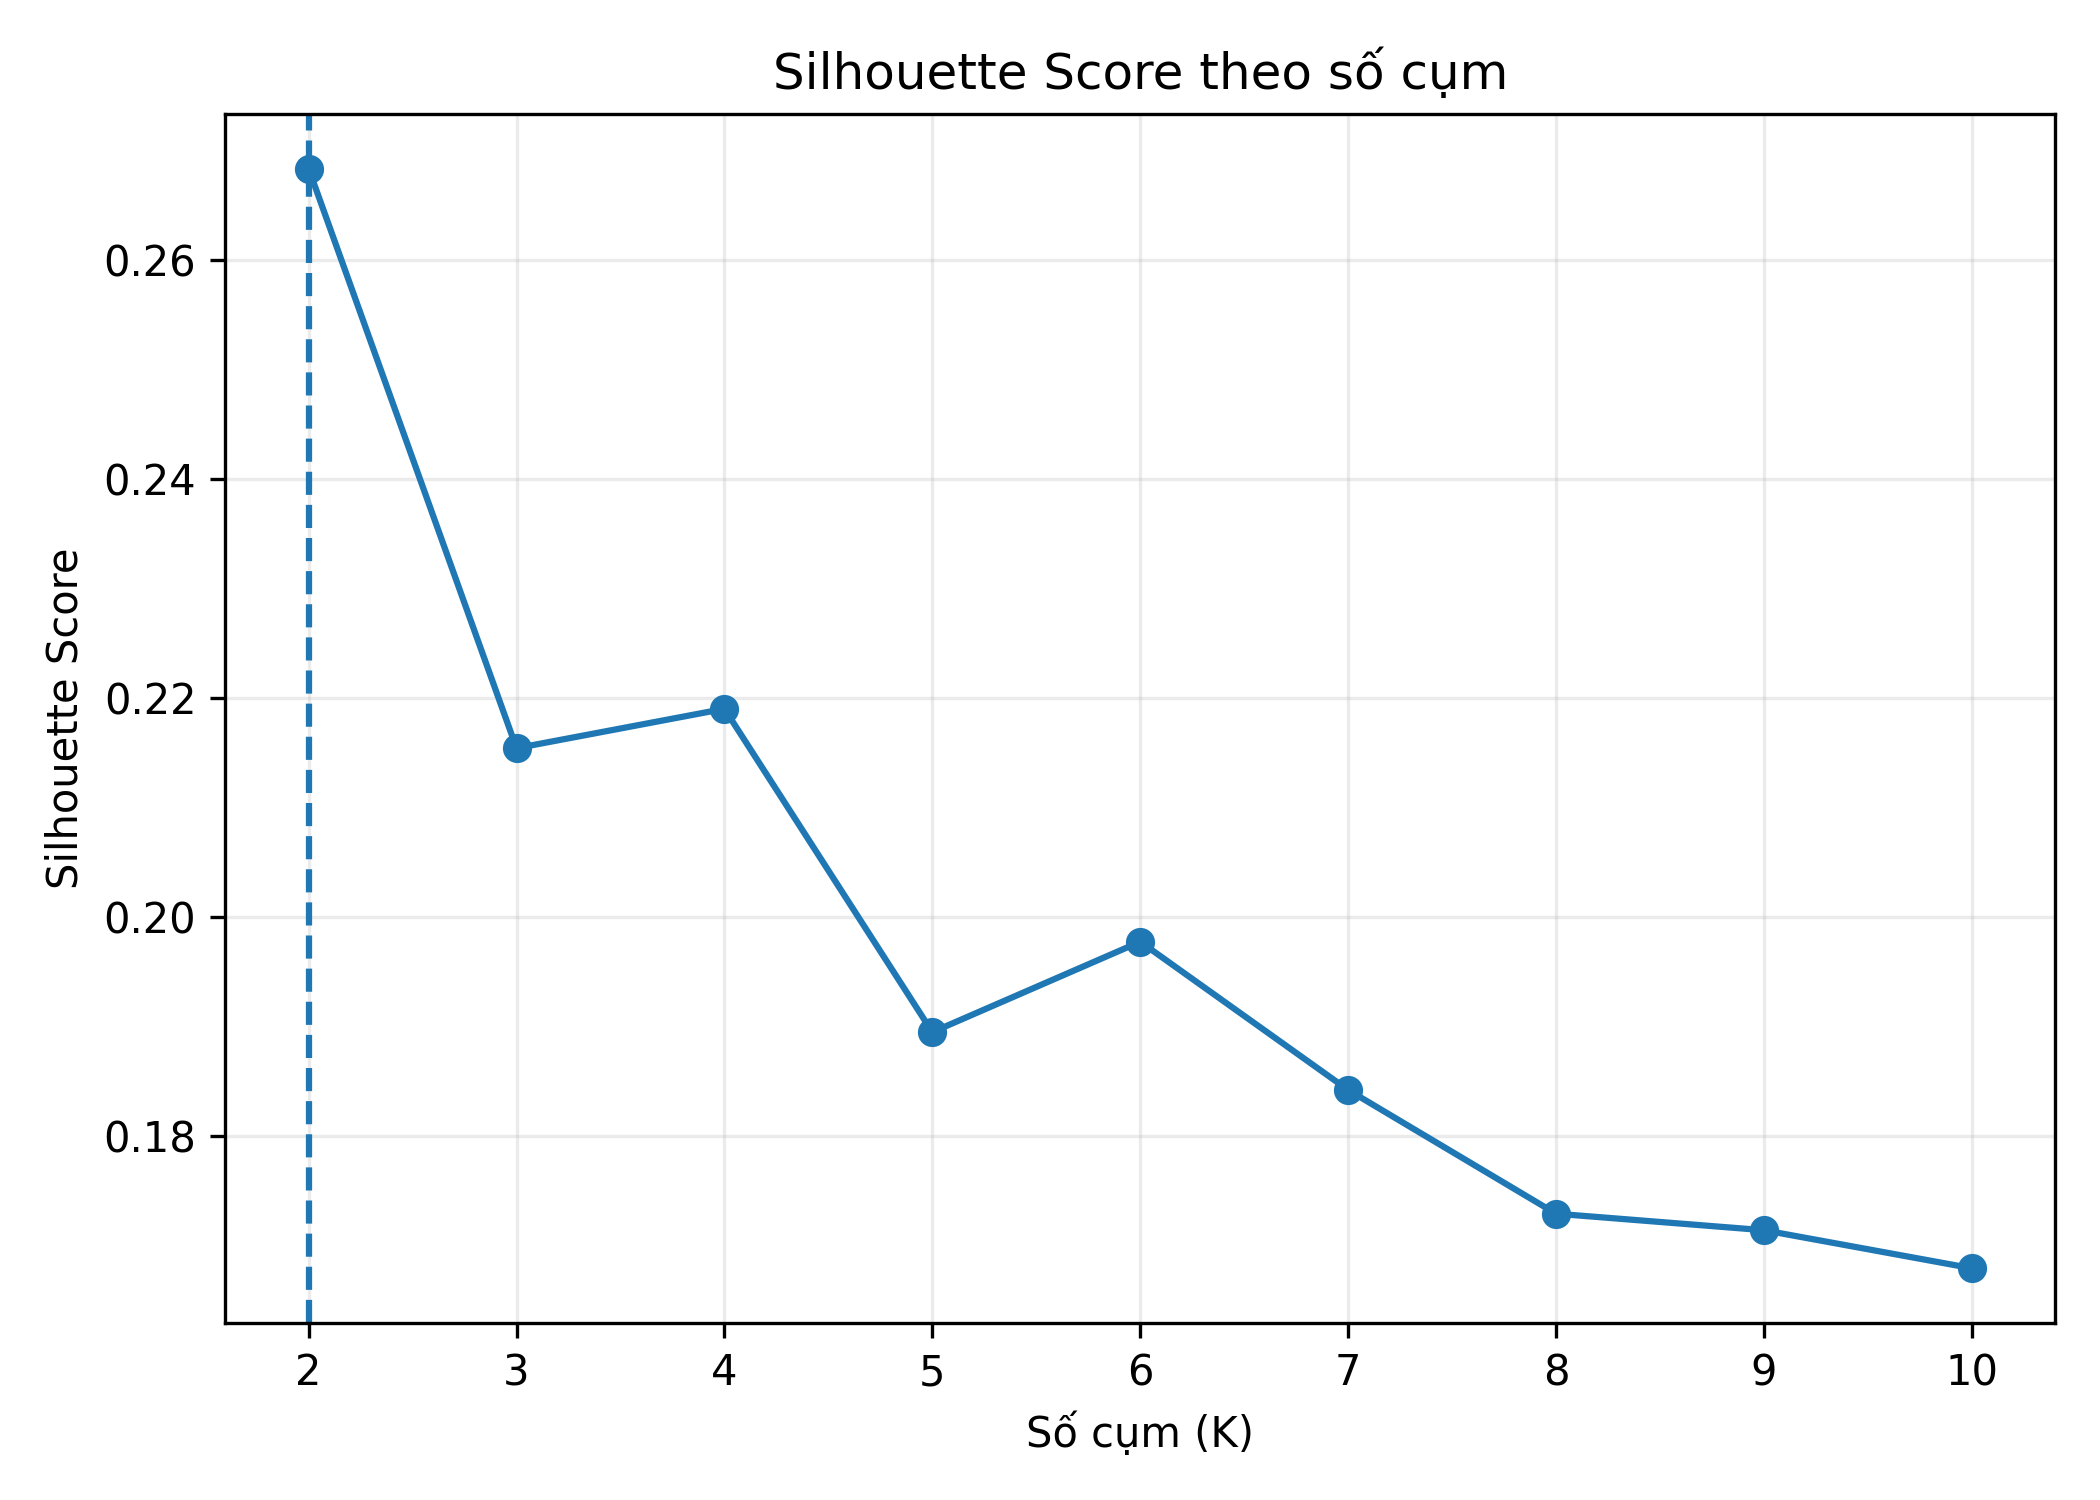
\includegraphics[width=0.7\textwidth]{images/anh_chuong4/kmeans_after_silhouette.png}
	\caption{\centering Silhouette Score của mô hình K-Means sau xử lý ngoại lai}
	\label{fig:kmeans_after_silhouette}
\end{figure}

Quan sát Hình \ref{fig:kmeans_after_elbow} và Hình \ref{fig:kmeans_after_silhouette} cho thấy WCSS giảm dần khi số cụm tăng, trong khi Silhouette Score đạt giá trị cao nhất tại \(K = 2\). Do đó, số cụm \(K = 2\) được lựa chọn để phân nhóm khách hàng sau xử lý ngoại lai.

\begin{figure}[H]
	\centering
	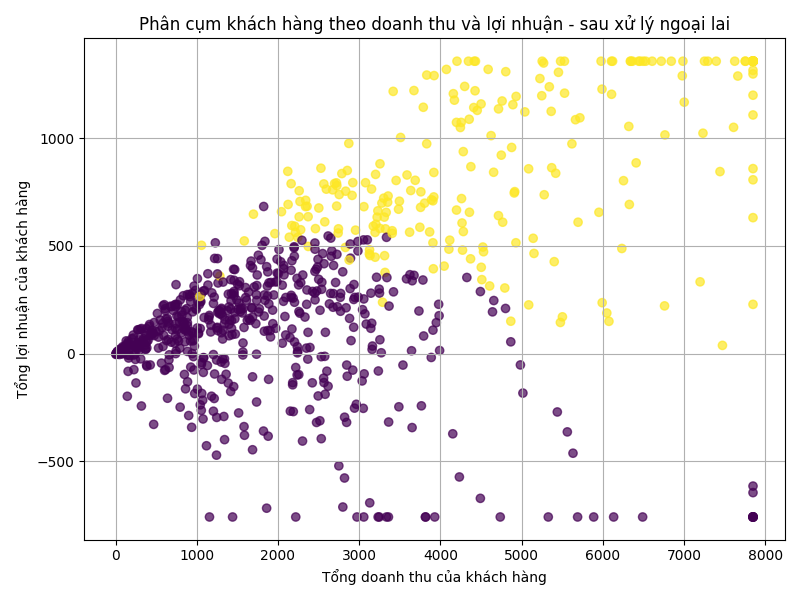
\includegraphics[width=0.8\textwidth]{images/anh_chuong4/kmeans_after_cluster.png}
	\caption{\centering Phân cụm khách hàng sau xử lý ngoại lai}
	\label{fig:kmeans_after_cluster}
\end{figure}

Quan sát Hình \ref{fig:kmeans_after_cluster} cho thấy các nhóm khách hàng được phân tách rõ ràng hơn so với trước xử lý ngoại lai. Một cụm tập trung nhiều khách hàng có doanh thu và lợi nhuận thấp hoặc trung bình, trong khi cụm còn lại đại diện cho nhóm khách hàng có giá trị cao hơn.

\begin{figure}[H]
	\centering
	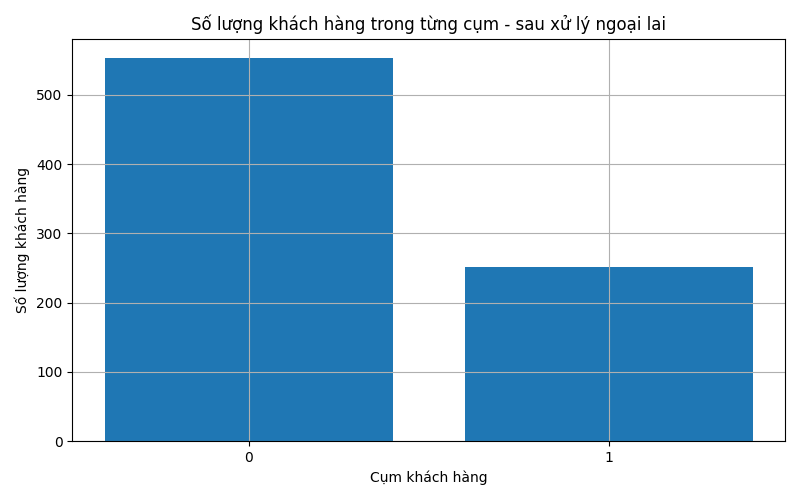
\includegraphics[width=0.65\textwidth]{images/anh_chuong4/kmeans_after_cluster_count.png}
	\caption{\centering Số lượng khách hàng trong từng cụm sau xử lý ngoại lai}
	\label{fig:kmeans_after_cluster_count}
\end{figure}

Biểu đồ số lượng khách hàng cho thấy hai cụm vẫn có sự chênh lệch về quy mô. Cụm 0 chiếm số lượng khách hàng lớn hơn, trong khi cụm 1 có ít khách hàng hơn nhưng thường đại diện cho nhóm có giá trị giao dịch cao hơn.

\begin{figure}[H]
	\centering
	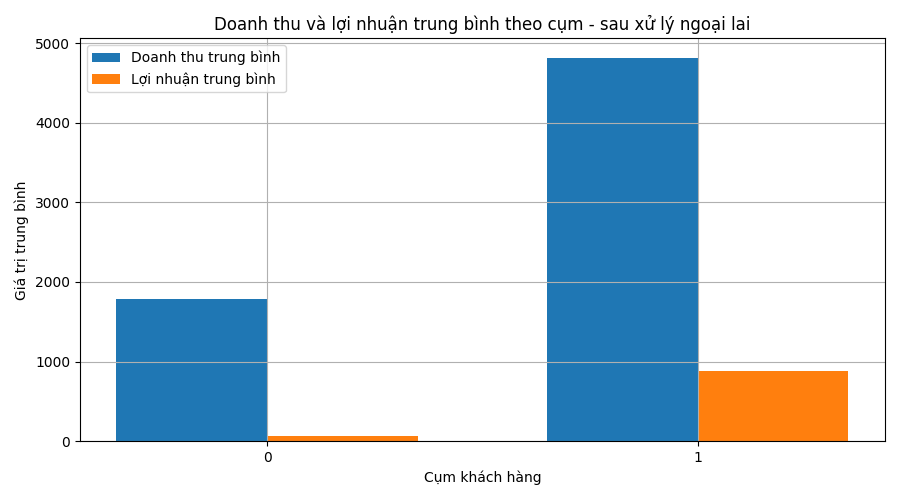
\includegraphics[width=0.75\textwidth]{images/anh_chuong4/kmeans_after_cluster_mean.png}
	\caption{\centering Doanh thu, lợi nhuận trung bình theo cụm sau xử lý ngoại lai}
	\label{fig:kmeans_after_cluster_mean}
\end{figure}

Quan sát Hình \ref{fig:kmeans_after_cluster_mean} cho thấy cụm 1 có doanh thu và lợi nhuận trung bình cao hơn rõ rệt so với cụm 0. Điều này cho thấy mô hình K-Means sau xử lý ngoại lai đã phản ánh tốt hơn sự khác biệt về giá trị giữa các nhóm khách hàng.

Nhìn chung, sau khi xử lý ngoại lai, kết quả phân cụm trở nên ổn định và dễ diễn giải hơn. Các cụm khách hàng không còn bị ảnh hưởng quá mạnh bởi các điểm dữ liệu cực đoan, từ đó hỗ trợ tốt hơn cho việc phân tích hành vi và giá trị khách hàng.

\refstepcounter{subsection}

\subsection*{\thesubsection\quad So sánh trước và sau xử lý ngoại lai}

Sau khi xử lý ngoại lai, kết quả phân cụm của mô hình K-Means trở nên ổn định và rõ ràng hơn. Các tâm cụm ít bị ảnh hưởng bởi các khách hàng có doanh thu hoặc lợi nhuận bất thường, giúp các cụm phản ánh chính xác hơn đặc điểm chung của từng nhóm khách hàng.

Ngoài ra, mức độ tách biệt giữa các cụm cũng được cải thiện sau khi dữ liệu được làm sạch. Điều này cho thấy việc xử lý ngoại lai giúp mô hình phân nhóm khách hàng hiệu quả hơn và nâng cao khả năng diễn giải kết quả.

Đối với K-Means, xử lý ngoại lai là bước quan trọng vì mô hình hoạt động dựa trên khoảng cách Euclid. Chỉ một số điểm dữ liệu cực đoan cũng có thể làm thay đổi vị trí tâm cụm và ảnh hưởng đến toàn bộ kết quả phân cụm. Vì vậy, việc kiểm soát ngoại lai giúp tăng độ tin cậy và tính ổn định của mô hình.

\refstepcounter{subsection}
\subsection*{\thesubsection\quad Nhận xét mô hình}

Kết quả phân cụm cho thấy khách hàng trong bộ dữ liệu có hành vi mua hàng và mức độ đóng góp lợi nhuận khác nhau. Một số nhóm khách hàng tạo ra doanh thu và lợi nhuận cao, trong khi một số nhóm khác có doanh thu tương đối lớn nhưng lợi nhuận thấp do ảnh hưởng của chiết khấu hoặc đặc điểm sản phẩm.

Điều này cho thấy doanh nghiệp không nên chỉ đánh giá khách hàng dựa trên doanh thu mà cần kết hợp thêm yếu tố lợi nhuận để xác định giá trị thực sự của từng nhóm khách hàng.

Kết quả của mô hình K-Means có ý nghĩa thực tiễn trong việc hỗ trợ phân khúc khách hàng và xây dựng chiến lược kinh doanh phù hợp. Doanh nghiệp có thể tập trung giữ chân nhóm khách hàng giá trị cao, đồng thời tối ưu chính sách chiết khấu và hoạt động bán hàng đối với các nhóm khách hàng có lợi nhuận thấp hơn.

